\documentclass[a4paper]{scrartcl}
\usepackage[english]{babel}
\usepackage[utf8]{inputenc}
\usepackage[T1]{fontenc}
\usepackage{ae}
\usepackage[pdftex,bookmarks=true,bookmarksnumbered,colorlinks=true]{hyperref} % http://ctan.org/pkg/hyperref
\usepackage{nameref}
\usepackage{comment} % for block commenting
\usepackage[table]{xcolor} % has to be loaded before tikZ
%%%%%%% package for sequence diagrams
\usepackage{tikz}
\usetikzlibrary{arrows,shadows}
\usepackage{../materials/resources/pgf-umlsd}
%%%%%%%
\usepackage{float}
\graphicspath{{../materials/images/design/}}
\usepackage[disable]{todonotes} % use temporary for todo notes
% \usepackage{lineno} % temporary use for correcting
\usepackage{xspace}
% \linenumbers
\usepackage{lipsum} % just to generate some text
\usepackage[nonumberlist,acronym,toc,section]{glossaries} % must be the last package to include

\setlength{\parindent}{0in}
\setlength{\parskip}{8pt}

\widowpenalty=10000 % Prevent single line after pagebreak
\clubpenalty=10000  % Prevent single line before pagebreak

% glossary
\makeglossaries
% Remove trailing dot
\renewcommand*{\glspostdescription}{}

%
% Glossary entries
%

\newglossaryentry{graphioli}{name=Graphioli,
description={A fancy name that combines \glspl{graph} with filled pasta.},
plural={Graphioli}}

\newglossaryentry{graph}{name=graph,
description={A (abstract) set of objects provided with binary relations.\\The objects of a graph are called \glspl{vertex} and are represented by nodes in the visualization. The relations are called \glspl{edge} and are represented by (in our case straight) lines between the respective vertices in a visualized graph.\todo{Passt so?}}}

\newglossaryentry{edge}{name=edge,
description={see \emph{\gls{graph}}}}

\newglossaryentry{vertex}{name=vertex,
description={see \emph{\gls{graph}}},
plural={vertices}}

\newglossaryentry{planar}{name=planar,
description={A \emph{planar} \gls{graph} is a graph that can be structure-preservingly redrawn in a way that no \glspl{edge} intersect.},
plural={planar}}

\newglossaryentry{planarity}{name=planarity,
description={see \emph{\gls{planar}}},
plural={planarities}}

\newglossaryentry{api}{name=application programming interface (API),
description={Set of routines and tools providing \gls{program} blocks, which are put together by a third-party programmer to ensure consistency with an existing program or \gls{framework}.}}

\newglossaryentry{gui}{name=graphical user interface (GUI),
description={\Gls{program} interface that uses a computer's graphical capabilities to provide easy access and handling for the program. It replaces the command-line based access.},
plural={graphical user interfaces (GUI)}}

\newglossaryentry{framework}{name=framework,
description={A layered structure indicating what kind of applications can or should be built and how they would interrelate. It specifies interfaces and reusable \glspl{program} that form the basis for such an application.}}

\newglossaryentry{java}{name=Java,
description={Java is a widely spread programming language originally developed by Sun Microsystems and released in 1995. Applications developed with Java are compiled into bytecode that runs on basically every system that has a \Gls{jvm} installed.},
plural={Java}}

\newglossaryentry{jvm}{name=Java Virtual Machine (JVM),
description={A virtual machine that can execute \Gls{java} byte code. Thus, the execution component of the Java platform.},
plural={Java Virtual Machines (JVM)}}

\newglossaryentry{jdk}{name=Java Development Kit (JDK),
description={A collection of programming tools for \Gls{java} developers.},
plural={Java Development Kit (JDK)}}

\newglossaryentry{jre}{name=Java Runtime Environment,
description={see \emph{\gls{jvm}}}}

\newglossaryentry{javadoc}{name=Javadoc,
description={Javadoc is a tool for generating API documentation in HTML format from doc comments in source code.\footnote{From Oracle, self-definition}},
plural={Javadoc}}

\newglossaryentry{customer}{name=customer,
description={A party that receives a copy of the created \gls{software} in order to use it for own implementations. The customer of this \gls{framework} will be the \gls{developer}.}}

\newglossaryentry{computer-game}{name=computer game,
description={An electronic game that requires the \gls{player}['s] interaction to influence its course of events. Such a game usually bases on graphical feedback.}}

\newglossaryentry{game}{name=game,
description={The implementation of a \gls{computer-game} that requires the usage of this \gls{framework}.}}

\newglossaryentry{network}{name=network,
description={A group of connected computers that are able to communicate and share data, e.g. for synchronizing \gls{game} statuses.}}

\newglossaryentry{tutorial}{name=tutorial,
description={Instructional document that provides step by step information about a specific topic or \gls{workflow}, e.g. how to start implementing your own \gls{game} using this \gls{framework}.}}

\newglossaryentry{editor}{name=editor,
description={see \emph{\gls{level-editor}}}}

\newglossaryentry{level-editor}{name=level editor,
description={An interface that lightens the \gls{developer}['s] workload at creating new levels.}}

\newglossaryentry{level}{name=level,
description={A stage of the current \gls{game}.}}

\newglossaryentry{player}{name=player,
description={One who plays one of the \glspl{game} developed by a \gls{developer} using this \gls{framework}.}}

\newglossaryentry{developer}{name=developer,
description={Someone who designs and implements \glspl{game} using the {\graphioli} framework.}}

\newglossaryentry{undo}{name=undo,
description={To restore a previous condition, e.g. a \gls{savegame} or the previous step in the \gls{level-editor}.}}

\newglossaryentry{redo}{name=redo,
description={Opposite of \emph{\gls{undo}}.}}

\newglossaryentry{four-color-theorem}{name=four color theorem,
description={In mathematics, the \emph{four color theorem} states that, given any separation of a plane into contiguous areas, no more than four colors are required to color these areas in a way that no two \gls{adjacent} areas have the same color.},
plural={four color theorem}}

\newglossaryentry{adjacent}{name=adjacent,
description={Two \glspl{vertex} connected by an \gls{edge} are called \emph{adjacent}.},
plural={adjacent}}

\newglossaryentry{program}{name=program,
description={see \emph{\gls{computer-program}}}}

\newglossaryentry{savegame}{name=savegame,
description={A data file that contains information about a current \gls{game} state and is created when saving a game. It allows the \gls{player} to jump to a previously reached level.}}

\newglossaryentry{computer-program}{name=computer program,
description={A sequence of instructions that a computer can interpret and execute.}}

\newglossaryentry{software}{name=software,
description={An organized collection of data and instructions for computers, that is used to accomplish specific tasks.\\A piece of software can consists of a single \gls{program} or a package of programs closely working together. Usually software is bundled with associated documentation.}}

\newglossaryentry{workflow}{name=workflow,
description={The sequence of administrative, technical, or other processes through which a \gls{software} project passes from initiation to completion.}}

\newglossaryentry{user}{name=user,
description={The \emph{user} of a \gls{software} is everybody how starts the \gls{program} in order to fulfill specified tasks.\\The user of this framework is the \gls{developer}, whereas the user of the final \gls{game} is the \gls{player} (see \ref{REF:HOW-TO-READ}).}}

\newglossaryentry{git}{name=Git,
description={A distributed revision control and source code management system developed by \emph{Linus Torvalds}. Every Git working directory is a full-fledged repository with complete history and full revision tracking capabilities, not dependent on network access or a central server.\footnote{From Wikipedia: Git (software), 08/05/2012}},
plural={Git}}

\newglossaryentry{eclipse}{name=Eclipse,
description={An open development platform comprised of extensible frameworks, tools and runtimes for building, deploying and managing software across the lifecycle.\footnote{From Eclipse project, self-definition}},
plural={Eclipse}}

\newglossaryentry{artificial-intelligence}{name=artificial intelligence (AI),
description={An intelligent system that perceives its environment and takes actions that maximize its chances of success.\footnote{Russell, Stuart J.; Norvig, Peter: Artificial Intelligence: A Modern Approach (2003, 2nd ed.)}\\An algorithm that tries to defeat its human counter-\glspl{player} in a \glspl{computer-game} could be referred to as \emph{artificial intelligence}.}}

\newglossaryentry{depth-first-search}{name=depth-first search (DFS),
description={An \gls{algorithm} for traversing or searching a \gls{graph}, starting at a selected root \gls{vertex} and exploring as far as possible along each branch before backtracking.\footnote{From Wikipedia: Breadth-first search, 08/05/2012}},
plural={depth-first searches (DFS)}}

\newglossaryentry{breadth-first-search}{name=breadth-first search (BFS),
description={An \gls{algorithm} for traversing or searching a \gls{graph}, starting at a selected root \gls{vertex} and inspecting all its neighboring vertices.},
plural={breadth-first searches (BFS)}}

\newglossaryentry{path}{name=path,
description={A sequence of \glspl{vertex} of a \gls{graph}.}}

\newglossaryentry{algorithm}{name=algorithm,
description={Procedure or set of (mathematical) rules for solving a problem in a finite number of steps, especially by a computer.}}

\newglossaryentry{library}{name=library,
description={A collection of resources used to develop \gls{software}. These may include pre-written code and subroutines, classes, values or type specifications.},
plural={libraries}}

\newglossaryentry{opensuse}{name=openSUSE,
description={A free and \Gls{linux}-based operating system.\footnote{From openSUSE Project, self-definition}},
plural={openSUSE}}

\newglossaryentry{linux}{name=Linux,
description={An alternative and open-source operating system for personal computers and servers.},
plural={Linuces}}

\newglossaryentry{metalanguage}{name=metalanguage,
description={Any (technical) language used to describe and define an implementation of a \gls{game} in the \gls{framework}. It substitutes the \Gls{java}-based programming of that implementation and can be parsed by the framework.}}

\newglossaryentry{mvc}{name=Model-View-Controller (MVC),
description={A design pattern for computer user interfaces describing the structural subdivision into the components `Model', `View' and `Controller'.},
plural={Model-View-Controllers (MVC)}}

\newglossaryentry{chat}{name=online chat,
description={A communication system over the internet.}}

%
% Acronyms
%

\newacronym{GUI}{GUI}{graphical user interface\protect\glsadd{gui}}

\newacronym{API}{API}{application programming interface\protect\glsadd{api}}

\newacronym{JVM}{JVM}{Java Virtual Machine\protect\glsadd{jvm}}

\newacronym{JDK}{JDK}{Java Development Kit\protect\glsadd{jdk}}

\newacronym{AI}{AI}{artificial intelligence\protect\glsadd{artificial-intelligence}}

\newacronym{DFS}{DFS}{depth-first search\protect\glsadd{depth-first-search}}

\newacronym{BFS}{BFS}{breadth-first search\protect\glsadd{breadth-first-search}}

\newacronym{MVC}{MVC}{Model-View-Controller\protect\glsadd{mvc}}

\newacronym{IDE}{IDE}{integrated development environment}

\newacronym{ID}{ID}{identification}

\author{Graphioli}
\title{Graphioli - Software Design Document}

\begin{document}
	
\setcounter{tocdepth}{5}
\setcounter{secnumdepth}{5}

\begin{titlepage}
\begin{center}
\fontsize{40}{50}\selectfont
        \vfill
        \textsc{Graphioli}
		\vfill
        \textsc{Functional Specification Document}
        \vfill
\LARGE
PSE SS 2012
  \vfill
 \newpage
 
 \null
 \vfill
 
 Praxis der Softwareentwicklung -- SS 2012 \\
 
  \Large
  Development of a Framework for Graph Games \\
  \medskip
  \vspace{2cm}
  
    Martin Dinh $\cdot$ Ole Fortmann $\cdot$ Leon Hielscher \\ Johannes Schäfer $\cdot$ Jack Unseld
  \vspace{2cm} \\
  \today
\end{center}

  \vfill

\end{titlepage}
\tableofcontents
\clearpage

% use this \textlabel command to have a reference within normal text; don't use any other referencing with textlabel enabled
\makeatletter
    \newcommand*{\textlabel}[2]{%
        \edef\@currentlabel{#1}% Set target label
        \leavevmode\phantomsection% Correct hyper reference link
        #1\label{#2}% Print and store label
    }
\makeatother

% proper nouns
\newcommand{\graphioli}{\textsc{Graphioli}\xspace}
\newcommand{\twixt}{\textsc {TwixT}\xspace}
\newcommand{\graphcoloring}{\textsc {Graph-Coloring}\xspace}

% creates the class name with its reference
\newcommand{\class}[2]{\subsubsection*{\textcolor{Blue}{Class \textlabel{#1}{cls:#2}}}}

% creates the interface name with its reference
\newcommand{\interface}[2]{\subsubsection*{\textcolor{Blue}{Interface \textlabel{#1}{cls:#2}}}}

% creates the abstract class name with its reference
\newcommand{\abstractclass}[2]{\subsubsection*{\textcolor{Blue}{Abstract Class \textlabel{#1}{cls:#2}}}}

% creates a reference for all implemented interfaces
\newcounter{iref}
\newcommand{\refi}[1]{\def\do##1{\stepcounter{iref}\ifnumgreater{\value{iref}}{1}{, }{}\ref{##1}}\docsvlist{#1}}

\newcommand{\interfaces}[1]{
	\begin{description}
		\item[All Implemented Interfaces] \hfill \\
		\refi{#1}
	\end{description}
	\setcounter{iref}{0}
}

% creates a reference for all direct subclasses
\newcounter{sref}
\newcommand{\reff}[1]{\def\do##1{\stepcounter{sref}\ifnumgreater{\value{sref}}{1}{, }{}\ref{##1}}\docsvlist{#1}}

\newcommand{\subclasses}[1]{
	\begin{description}
		\item[Direct Known Subclasses] \hfill \\
		\reff{#1}
	\end{description}
	\setcounter{sref}{0}
}

% create centered dashed rule
\newcommand{\centerdash}{
	\begin{center}
		\hdashrule{14cm}{1pt}{1pt}
	\end{center}
}

% to easily implement methods
\newcommand{\method}[3]{#1 & \textcolor{NavyBlue}{\textlabel{#2}{#3}}} 

% creates the beginning of the method description table
\newcommand{\startmethodtable}{\hline\rowcolor{white}\textbf{Modifier and Type} & \textbf{Method and Description} \\ \hline}

\section{Introduction}
Game premised on graph algorithm have always been played as a pastime. Mostly without the knowledge about the underlying mathematical theories, which are -- of course -- not always relevant for clearing level after level. While two humans playing a graph game usually agree on the eventuation of one player winning the game, the same game on a computer must be computed to declare one player the winner.\par

This is where \graphioli takes effect. The Java framework simplifies the process of developing graph-based computer games by providing a straightforward, intuitive library that allows its user to focus the effort to the game's logical implementation. Recurring and redundant operations, algorithms and codings will be taken care of by \graphioli.\par

The framework still does not release the developer from actual programming work. However, it reduces the amount of time formerly spent realizing graphical outputs, structures and user interactions, thus reinventing the wheel.\par

Products based on \graphioli will be well-structured, lightweight in terms of code size and easy to maintain.\par

\subsection{About this document}
This document developed during validation and quality assurance phase and is divided into three parts:\par
In Section \ref{section:tests} we introduce the four different types of tests conducted: Unit tests, algorithm regressions tests, GUI tests and the manual test cases and scenarios.\par
Section \ref{section:results} describes the concrete tests and outlines their outcomes in tables and lists. Statistics about results and code coverage are provided.\par
The last section, Section \ref{section:corrected-errors}, documents the errors that were corrected during the phase.\par
\section{Architecture}
The \graphioli framework realizes the \gls{MVC} design pattern in which the classes are separated by their function in either `Model', `View' and `Controller'.\par
This is achieved by the following design:\par

\begin{description}
	\item[Model] The model contains the \ref{cls:gameboard} that serves as a mediator between the logical \gls{graph} (\ref{cls:graph}) and the visual graph on a \gls{grid} (\ref{cls:grid}).
	\item[View] An implementation of the \gls{interface} \ref{cls:view} is responsible for output and capturing user interactions.
	\item[Controller] The controller is divided into three parts. \ref{cls:gamemanager} conducts the basic game operations and interacts extensively with the class that inherits from \ref{cls:game} (not part of the framework). The \ref{cls:viewmanager} maintains consistency with the \emph{View}.
\end{description}

\begin{figure}[h]
	\centering
	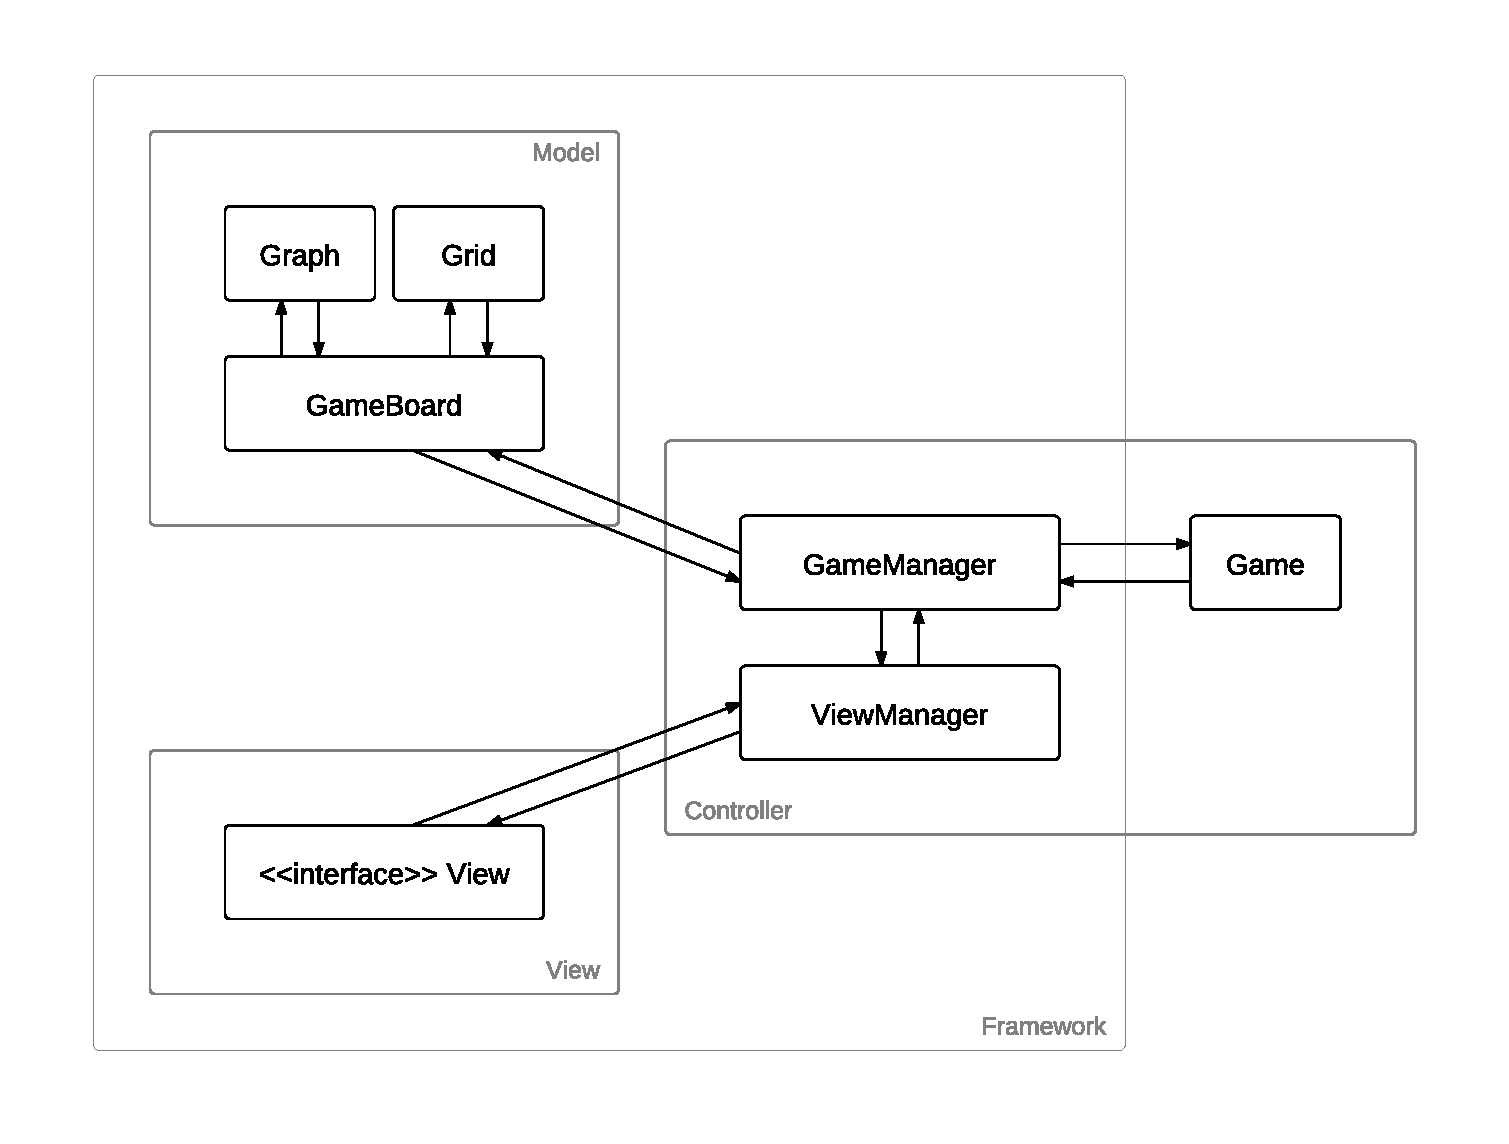
\includegraphics[width=1\textwidth]{archMVC.pdf}
	\caption{Diagram showing the realization of the \gls{MVC} design pattern by the framework.}
	\label{img:archMVC}
\end{figure}
\section{Class Diagram}

\begin{figure}[h]
	\centering
	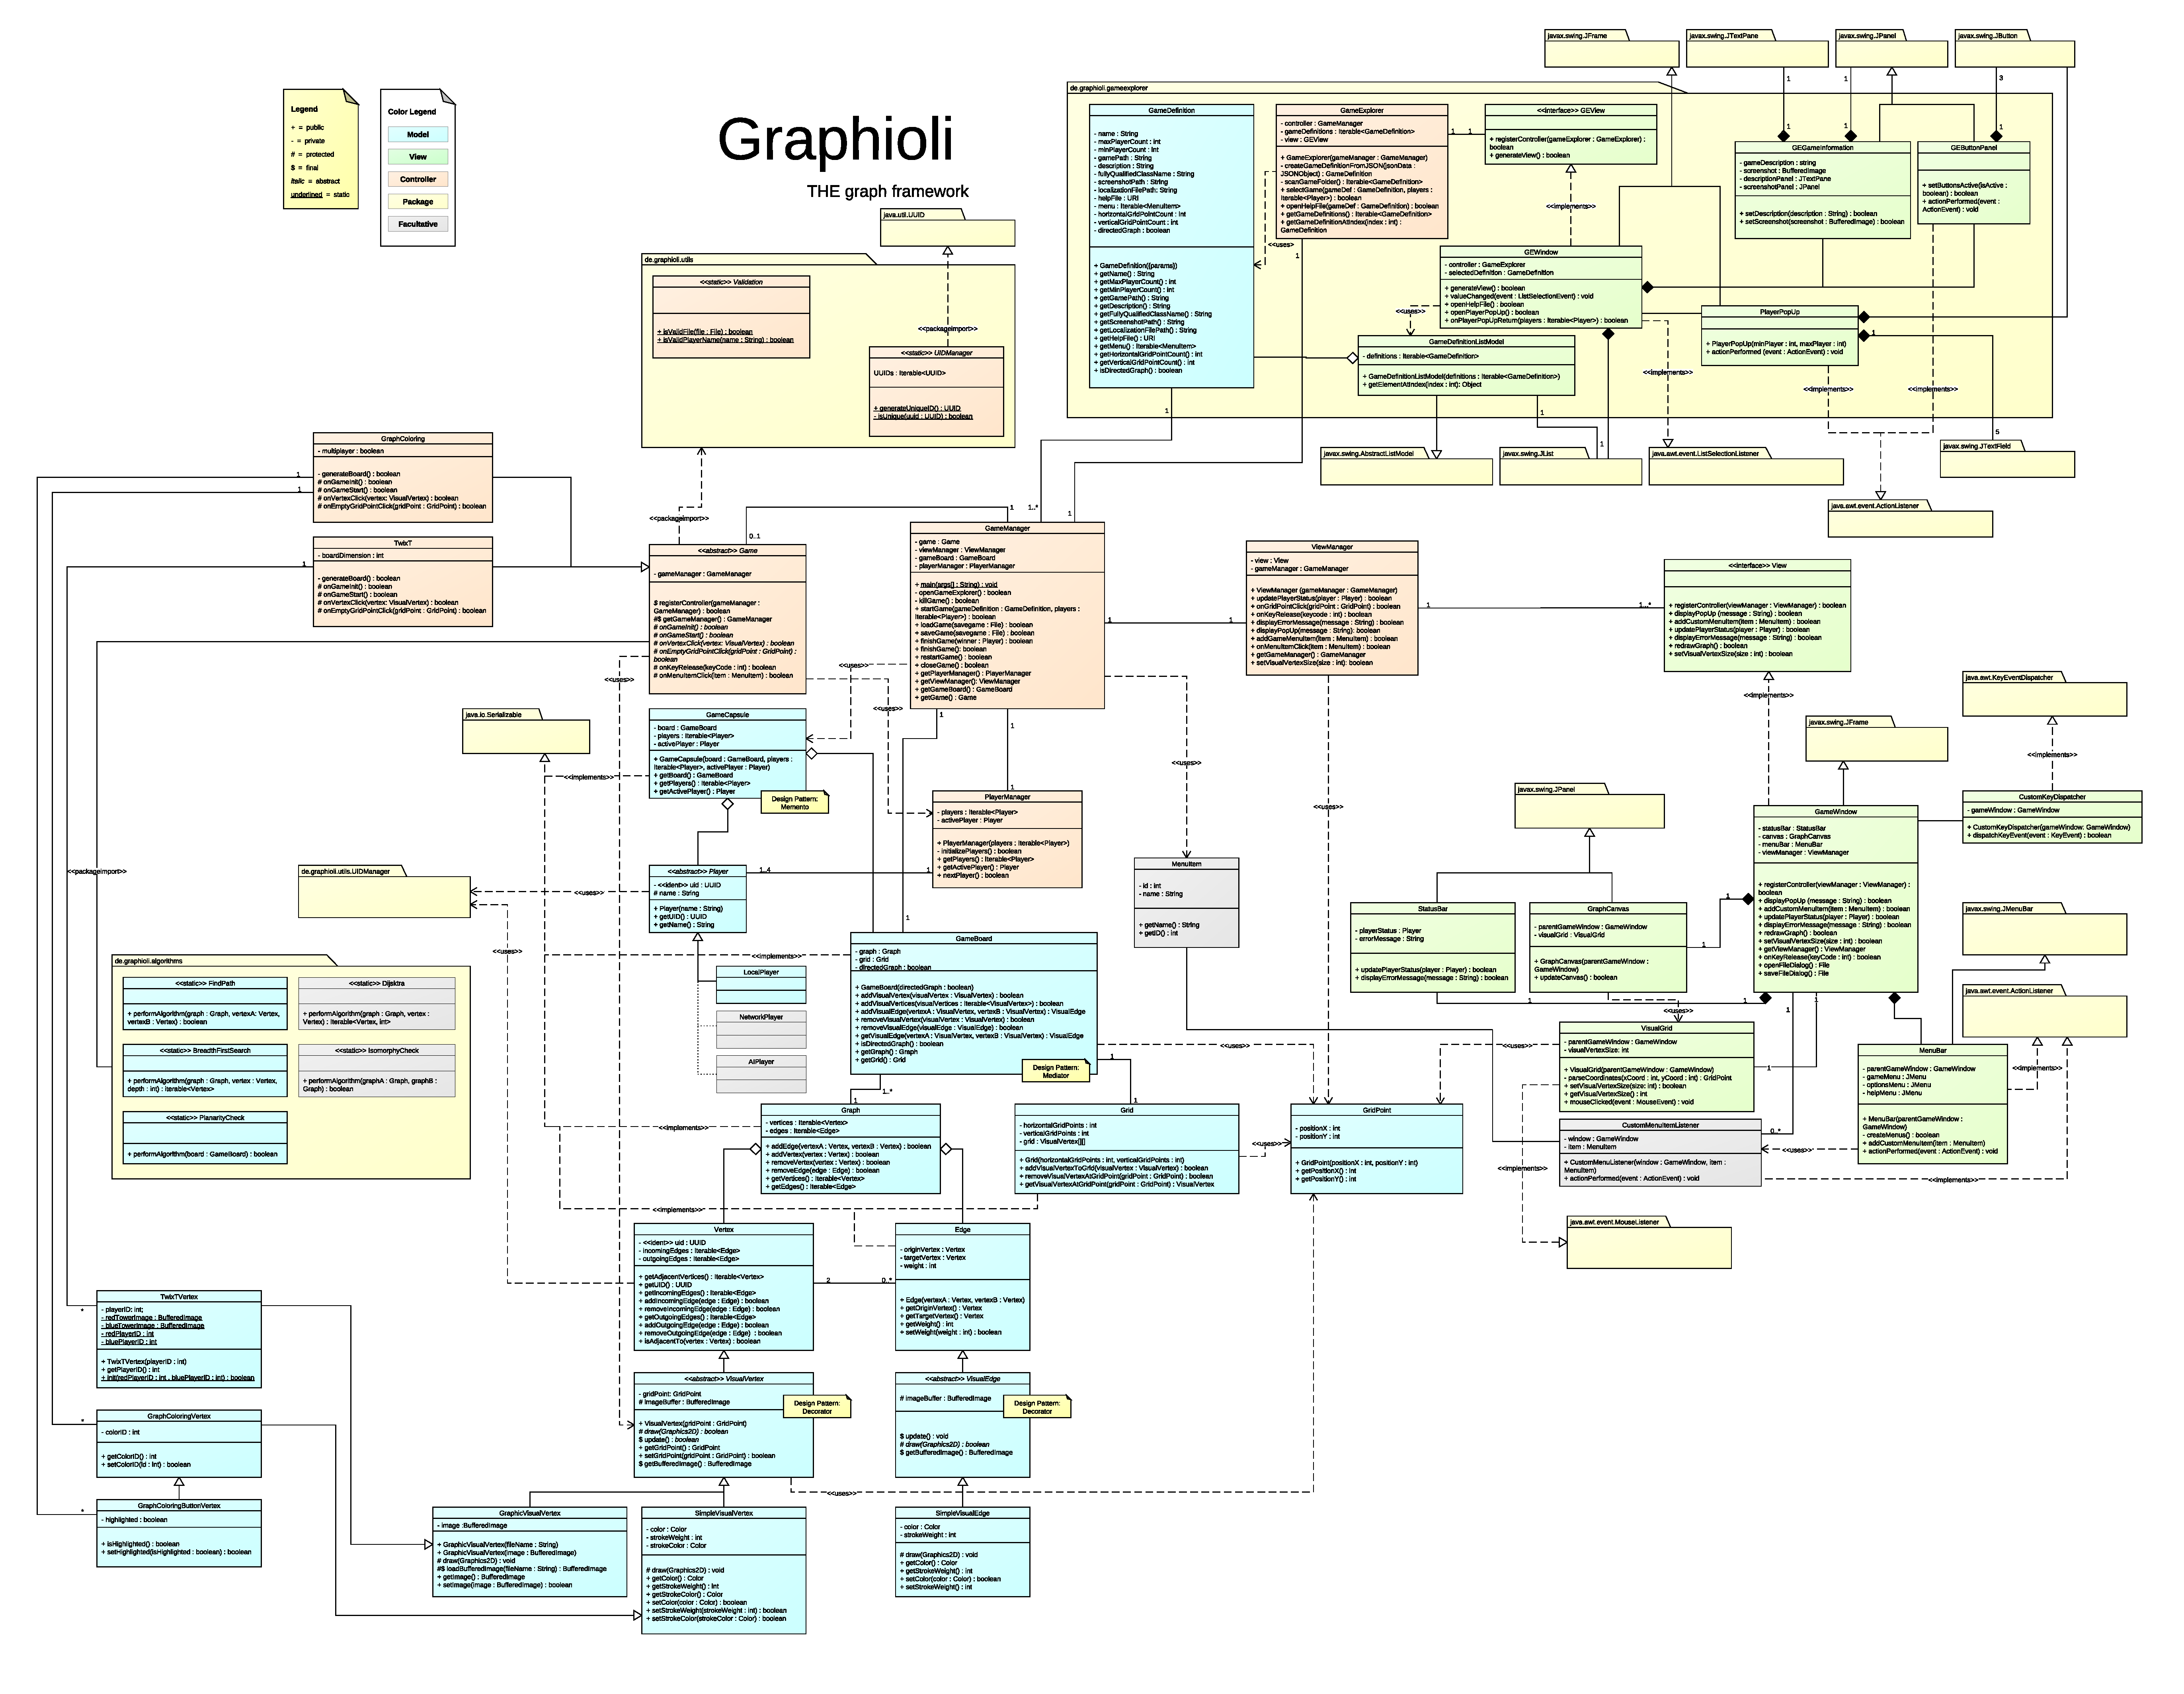
\includegraphics[angle=90,width=0.78\textwidth,keepaspectratio]{classGraphioli.pdf}
	\caption{Class diagram showing the framework's inter-class dependencies. The MVC design pattern is outlined by different colors.}
	\label{img:classGraphioli}
\end{figure}
\section{Class Description}
\subsection{Model}

% Graph
\subsubsection*{\textcolor{Blue}{Class \textlabel{Graph}{cls:graph}}}
%\createindentedlist{string1,string2,string3}
This class represents the logical graph. \\
\begin{description}
	\item[Direct Known Subclasses] \hfill \\
	\ref{cls:vertex}, \ref{cls:edge}
\end{description}
\vspace{.5cm}
\hrule
\paragraph*{Method Summary}
\paragraph*{}
\begin{longtable}{Lp{10cm}}
	\hline
    \rowcolor{white}\textbf{Modifier and Type} & \textbf{Method and Description} \\ \hline
	\method{public boolean}{addEdge(Vertex vertexA, Vertex vertexB)}{graph:addEdge} \\
	& Adds an \ref{cls:edge} to this graph. \\
	\method{public boolean}{addVertex(vertex : Vertex)}{graph:addVertex} \\
	& Adds a \ref{cls:vertex} to this graph. \\
	\method{public boolean}{removeVertex(Vertex vertex)}{graph:removevertex} \\
	& Removes a specified \ref{cls:vertex} from this graph. \\
	\method{public boolean}{removeEdge(Edge edge)}{graph:removeedge} \\
	& Removes a specified \ref{cls:edge} from this graph. \\
	\method{public Iterable<Vertex>}{getVertices()}{graph:iterablevertex} \\
	& Returns an iterable list of vertices.  \\
	\method{public Iterable<Edge>}{getEdge()}{graph:iterableedge} \\
	& Returns an iterable list of vertices. \\
	\hline
\end{longtable}

\setcounter{row}{-1}

% Vertex
\subsubsection*{\textcolor{Blue}{Class \textlabel{Vertex}{cls:vertex}}}
This class represents the logical vertex. \\
\begin{description}
	\item[Direct Known Subclasses] \hfill \\
	\ref{cls:visualvertex}
\end{description}
\vspace{.5cm}
\hrule
\paragraph*{Method Summary}
\paragraph*{}
\begin{longtable}{Lp{10cm}}
	\hline
    \rowcolor{white}\textbf{Modifier and Type} & \textbf{Method and Description} \\ \hline
	\method{public Iterable<Vertex>}{getAdjacentVertices()}{vertex:getadjacentvertices} \\
	& Returns all vertices that are connected to this vertex. \\
	\method{public UUID}{getUID()}{vertex:getuid} \\
	& Returns the unique identifier for this vertex. \\
	\method{public Iterable<Edge>}{getInboundEdges()}{vertex:getinboundedges} \\
	& Returns an iterable list of inbound edges. \\
	\method{public boolean}{addInboundEdge(Edge edge)}{vertex:addinboundedge} \\
	& Adds an inbound \ref{cls:edge} to the list of inbound edges. \\
	\method{public Iterable<Edge>}{getOutboundEdges()}{vertex:getoutboundedges} \\
	& Returns an iterable list of outbound edges. \\
	\method{public boolean}{addOutboundEdge(Edge edge)}{vertex:addoutboundedge} \\
	& Adds an outbound \ref{cls:edge} to the list of outbound edges. \\
	\method{public boolean}{isAdjacentTo(Vertex vertex)}{vertex:isadjacentto} \\
	\hline
\end{longtable}

% VisualVertex
\subsubsection*{\textcolor{Blue}{Class \textlabel{VisualVertex}{cls:visualvertex}}}
This class represents a \ref{visualvertex}. \\
Dependencies: \textit{extends \ref{vertex}}
\paragraph*{Method Summary}
\paragraph*{}
\begin{longtable}{Lp{10cm}}
	\hline
    \rowcolor{white}\textbf{Modifier and Type} & \textbf{Method and Description} \\ \hline
	public & \textcolor{NavyBlue}{\textlabel{VisualVertex(gridPoint : GridPoint)}{vv:constructor}} \\
	& Creates a new VisualVertex and places it on the specified \ref{gridpoint}. \\
	protected void & \textcolor{NavyBlue}{\textlabel{draw(Graphics2D)}{vv:draw}} \\
	& Draws the VisualVertex. \\
	final void & \textcolor{NavyBlue}{\textlabel{update()}{vv:update}} \\
	& Updated the VisualVertex. \\ 
	public \ref{gridpoint} & \textcolor{NavyBlue}{\textlabel{getGridPoint()}{vv:getgridpoint}}\\
	& Returns the GridPoint of the VisualVertex. \\ 
	public boolean & \textcolor{NavyBlue}{\textlabel{setGridPoint(gridPoint : GridPoint)}{vv:setGridPoint(gridPoint : GridPoint)}} \\
	& Sets the GridPoint of the VisualVertex. \\
	public BufferedImage & \textcolor{NavyBlue}{\textlabel{getBufferedImage()}{vv:getbufferedimage}} \\
	& Returns the BufferedImage on the VisualVertex \\ \hline
\end{longtable}
\subsubsection{Algorithm Classes}

% FindPath
\static{FindPath}{findpath}
This class is part of the \texttt{de.graphioli.algorithms} package and is able to check if there is a path between two given \texttt{vertices}. \\

\centerdash

\paragraph*{Method Summary}
\paragraph*{}
\begin{longtable}{Lp{10cm}}
	\startmethodtable
	\method{public boolean}{performAlgorithm(Graph graph, Vertex vertexA, Vertex vertexB)}{fp:performalgorithm} \\
	& Returns \texttt{true} if there is a path in the specified \ref{cls:graph} between the two specified \texttt{vertices} \texttt{vertexA} and \texttt{vertexB}. \\
	\hline
\end{longtable}

% BreadthFirstSearch
\static{BreadthFirstSearch}{breadthfirstsearch}
This class is part of the \texttt{de.graphioli.algorithms} package and is able to perform the \gls{BFS} algorithm. \\

\centerdash

\paragraph*{Method Summary}
\paragraph*{}
\begin{longtable}{Lp{10cm}}
	\startmethodtable
	\method{public Iterable<Vertex>}{performAlgorithm(Graph graph, Vertex vertex, int depth)}{bfs:performalgorithm} \\
	& Performs the \gls{BFS} algorithm on the specified \ref{cls:graph} with the specified \ref{cls:vertex} and \texttt{depth}, and returns an iterable list of  traveled \texttt{vertices}. \\
	\hline
\end{longtable}

% PlanarityCheck
\static{PlanarityCheck}{planaritycheck}
This class is part of the \texttt{de.graphioli.algorithms} package and is able to check if a drawn \ref{cls:graph} is planer. \\

\centerdash

\paragraph*{Method Summary}
\paragraph*{}
\begin{longtable}{Lp{10cm}}
	\startmethodtable
	\method{public boolean}{performAlgorithm(GameBoard board)}{pc:performalgorithm} \\
	& Returns \texttt{true} if the specified \ref{cls:gameboard} is drawn planarly. \\
	\hline
\end{longtable}
\subsection{Controller}

\begin{figure}[h]
	\centering
	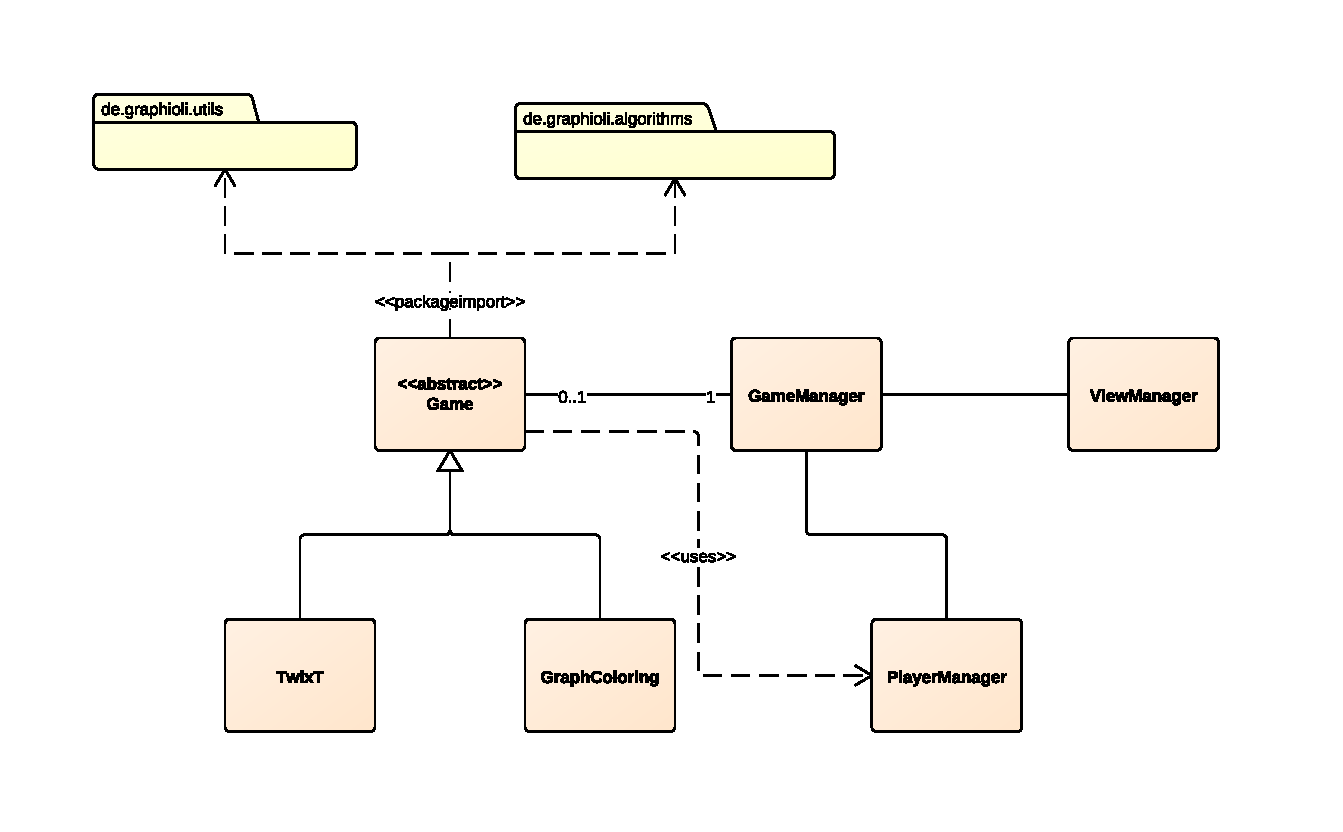
\includegraphics[page=1,width=\textwidth,keepaspectratio]{controllerClassDiagram.pdf}
	\caption{Controller class diagram.}
	\label{img:controllerClassDiagram}
\end{figure}

\pagebreak

% Game
\abstractclass{Game}{game}
This is the class that every \gls{game} has to inherit from, when using the \graphioli framework. It defines the callback functions that the game developer needs in order to implement the game's logic. \\

\subclasses{cls:graphcoloring, cls:twixt}

\centerdash

\paragraph*{Method Summary}
\paragraph*{}
\begin{longtable}{Lp{10cm}}
	\startmethodtable
	\method{public final boolean}{registerController(GameManager manager)}{game:registercontroller} \\
	& Associates this \texttt{Game} with a \ref{cls:gamemanager}. \\
	\method{protected final GameManager}{getGameManager()}{game:getgamemanager} \\
	& Returns the associated \ref{cls:gamemanager}. \\
	\method{protected abstract boolean}{onVertexClick(VisualVertex vertex)}{game:onvertexclick} \\
	& Called when a player clicks on a \ref{cls:visualvertex}. \\
	\method{protected abstract boolean}{onEmptyGridPointClick(GridPoint gridPoint)}{game:onemptygridpointclick} \\
	& Called when a player clicks on a \ref{cls:gridpoint} that has no \ref{cls:visualvertex} on it. \\
	\method{protected abstract boolean}{onGameInit()}{game:ongameinit} \\
	& Called after a \texttt{Game} has been instantiated. \\
	\method{protected abstract boolean}{onGameStart()}{game:ongamestart} \\
	& Called immediately before a \texttt{Game} gets (re)started. \\
	\method{protected boolean}{onKeyRelease(int keyCode)}{game:onkeyrelease} \\
	& Called when a player releases a keyboard key.\\
	\method{protected boolean}{onMenuItemClick(MenuItem item)}{game:onmenuitemclick} \\
	& Called when a player clicks on a custom \texttt{MenuItem}. \\
	\hline
\end{longtable}

\pagebreak

% GameManager
\class{GameManager}{gamemanager}
This is the framework's central class, connecting the actual game with the \texttt{model} and the \texttt{view}. Any communication between \texttt{model}, \texttt{view} and \texttt{controller} will be managed by the \texttt{GameManager}. \\

\centerdash

\paragraph*{Method Summary}
\paragraph*{}
\begin{longtable}{Lp{10cm}}
	\startmethodtable
	\method{public static void}{main(String[ ] args)}{gm:main} \\
	& The main method initializes the \texttt{GameManager} to start the whole application. \\
	\method{private boolean}{openGameExplorer()}{gm:opengameexplorer} \\
	& Starts the \ref{cls:gameexplorer}. \\
	\method{private boolean}{killGame()}{gm:killgame} \\
	& Kills the currently running game. \\
	\method{public boolean}{startGame(GameDefinition gameDefinition)}{gamemanager:startgame} \\
	& Starts the game specified by the \ref{cls:gamedefinition}. \\
	\method{public boolean}{loadGame(File savegame)}{gm:loadgame} \\
	& Creates a \ref{cls:gamecapsule} from the savegame file and loads the information to start the game in the saved state. \\
	\method{public boolean}{saveGame(File savegame)}{gm:savegame} \\
	& Creates a \ref{cls:gamecapsule} and serializes it into a savegame file to save the current state of the game. \\
	\method{public boolean}{finishGame()}{gm:finishgame} \\
	& Finishes the game and displays a default pop-up for single player games. \\
	\method{public boolean}{finishGame(Player winner)}{gm:finishgameWinner} \\
	& Finishes the game and displays the winning \ref{cls:player} in a pop-up.  \\
	\method{public boolean}{restartGame()}{gm:restartgame} \\
	& Restarts the game and resets the \ref{cls:gameboard} and \ref{cls:player}s. \\
	\method{public boolean}{closeGame()}{gm:closegame} \\
	& Closes the game with its \ref{cls:gamewindow} and returns the focus to the \ref{cls:gameexplorer}. \\
	\method{public PlayerManager}{getPlayerManager()}{gm:getplayermanager} \\
	& Returns the \ref{cls:playermanager} associated with this \texttt{GameManager}.\\
	\method{public ViewManager}{getViewManager()}{gm:getviewmanager} \\
	& Returns the \ref{cls:viewmanager} associated with this \texttt{GameManager}.\\
	\method{public GameBoard}{getGameBoard()}{gm:getgameboard} \\
	& Returns the \ref{cls:gameboard} associated with this \texttt{GameManager}.\\
	\hline
\end{longtable}

\pagebreak

% ViewManager
\class{ViewManager}{viewmanager}
This class acts as an interface between the \gls{GUI} and the other parts of the \gls{framework}. It pushes update notifications to the view and receives user input from it. \\

\centerdash

\paragraph*{Method Summary}
\paragraph*{}
\begin{longtable}{Lp{10cm}}
	\startmethodtable
	\method{public}{ViewManager(GameManager gameManager)}{viewmanager:viewmanager} \\
	& Creates a new \texttt{ViewManager} associated with the given \ref{cls:gamemanager}. \\
	\method{public boolean}{updatePlayerStatus(Player player)}{viewmanager:updateplayerstatus} \\
	& Notifies the \ref{cls:view} to display the given \ref{cls:player} as active. \\
	\method{public boolean}{onGridPointClick(GridPoint gridpoint)}{viewmanager:ongridpointclick} \\
	& Callback function used by the \ref{cls:view} to notify about a click on a \ref{cls:gridpoint}.  \\
	\method{public boolean}{onKeyRelease(int keycode)}{viewmanager:onkeyrelease} \\
	& Callback function used by the \ref{cls:view} to notify about a key release. \\
	\method{public boolean}{displayErrorMessage(String message)}{viewmanager:displayerrormessage} \\
	& Notifies the \ref{cls:view} to display the error message. \\
	\method{public boolean}{displayPopUp(String message)}{viewmanager:displaypopup} \\
	& Notifies the \ref{cls:view} to display the given message in a pop-up. \\
	\method{public boolean}{addGameMenuItem(MenuItem item}{viewmanager:addgamemenuitem} \\
	& Notifies the \ref{cls:view} to add the given \texttt{MenuItem} to the menu. \\
	\method{public boolean}{onMenuItemClick(MenuItem item)}{viewmanager:onmenuitemclick} \\
	& Callback function used by the \ref{cls:view} to notify about a click on a previously added \texttt{MenuItem}.  \\
	\method{public GameManager}{getGameManager()}{viewmanager:getgamemanager} \\
	& Returns the associated \ref{cls:gamemanager}. \\
	\method{public boolean}{setVisualVertexSet(int size)}{viewmanager:setvisualvertexsize} \\
	& Notifies the \ref{cls:view} to change the \texttt{size} of the \texttt{VisualVertices} to the given value. \\
	\hline
\end{longtable}

\pagebreak

% PlayerManager
\class{PlayerManager}{playermanager}
This class is responsible for keeping information about a game's \ref{cls:player}s.  \\

\centerdash

\paragraph*{Method Summary}
\paragraph*{}
\begin{longtable}{Lp{10cm}}
	\startmethodtable
	\method{public}{PlayerManager(Iterable<Player> players)}{pm:playermanager} \\
	& Constructs a \texttt{PlayerManager} with the given set of \ref{cls:player}s. \\
	\method{private boolean}{initializePlayers()}{pm:initializeplayers} \\
	& Initializes registered \ref{cls:player}s. \\
	\method{public Iterable<Player> players}{getPlayers()}{pm:getplayers} \\
	& Returns the list of \ref{cls:player}s managed by this instance. \\
	\method{public Player}{getActivePlayer()}{pm:getactiveplayer} \\
	& Returns the \ref{cls:player}, who is currently active. \\
	\method{public Player}{nextPlayer()}{pm:nextplayer} \\
	& Sets the next \ref{cls:player} in the list to active. \\
	\hline
\end{longtable}

\pagebreak

\subsubsection{Games}

%GraphColoring
\class{GraphColoring}{graphcoloring}
\createindentedlist{de.graphioli.controller.Game, de.graphioli.controller.GraphColoring}
Our implemented game containing the game's logic of \graphcoloring in single and multiplayer mode. \\

\centerdash

\paragraph*{Method Summary}
\paragraph*{}
\begin{longtable}{Lp{10cm}}
	\startmethodtable
	\method{private boolean}{generateBoard()}{gc:generateboard} \\
	& Generates the \ref{cls:gameboard} used to play the game. \\
	\method{protected abstract boolean}{onVertexClick(VisualVertex vertex)}{gc:onvertexclick} \\
	& Colors the given \ref{cls:vertex} -- if possible -- and decides if the game is finished by this move. \\
	\method{protected abstract boolean}{onEmptyGridPointClick(GridPoint gridPoint)}{gc:onemptygridpointclick} \\
	& Has no function in this game. \\
	\method{protected abstract boolean}{onGameInit()}{gc:ongameinit} \\
	& Decides whether the game is started in \texttt{single} or \texttt{multiplayer mode}. \\
	\method{protected abstract boolean}{onGameStart()}{gc:ongamestart} \\
	& (Re)builds the \ref{cls:gameboard} using \ref{gc:generateboard}. \\
	\hline
\end{longtable}

\pagebreak

%TwixT
\class{TwixT}{twixt}
\createindentedlist{de.graphioli.controller.Game, de.graphioli.controller.TwixT}
Our implemented game containing the game's logic of \twixt. \\

\centerdash

\paragraph*{Method Summary}
\paragraph*{}
\begin{longtable}{Lp{10cm}}
	\startmethodtable
	\method{private boolean}{generateBoard()}{twixt:generateboard} \\
	& Generates the \ref{cls:gameboard} used to play the game. \\
	\method{protected abstract boolean}{onVertexClick(VisualVertex vertex)}{twixt:onvertexclick} \\
	& Selects a tower on the \ref{cls:gameboard} and creates an \ref{cls:edge} between this \ref{cls:vertex} and the one previously selected if they belong to the same \ref{cls:player} and the new \ref{cls:edge} would not intersect with another one.
	It then checks if the baselines are connected and the game is finished.\\
	\method{protected abstract boolean}{onEmptyGridPointClick(GridPoint gridPoint)}{twixt:onemptygridpointclick} \\
	& Sets a new \ref{cls:twixtvertex} belonging to the active \ref{cls:player} onto the given \ref{cls:gridpoint}, if possible. \\
	\method{protected abstract boolean}{onGameInit()}{twixt:ongameinit} \\
	& Initilaizes the \ref{cls:twixtvertex} class. \\
	\method{protected abstract boolean}{onGameStart()}{twixt:ongamestart} \\
	& (Re)builds the \ref{cls:gameboard} using \ref{twixt:generateboard}. \\	
	\hline
\end{longtable}
\subsection{View}
\subsection{Game Explorer}

\begin{figure}[h]
	\centering
	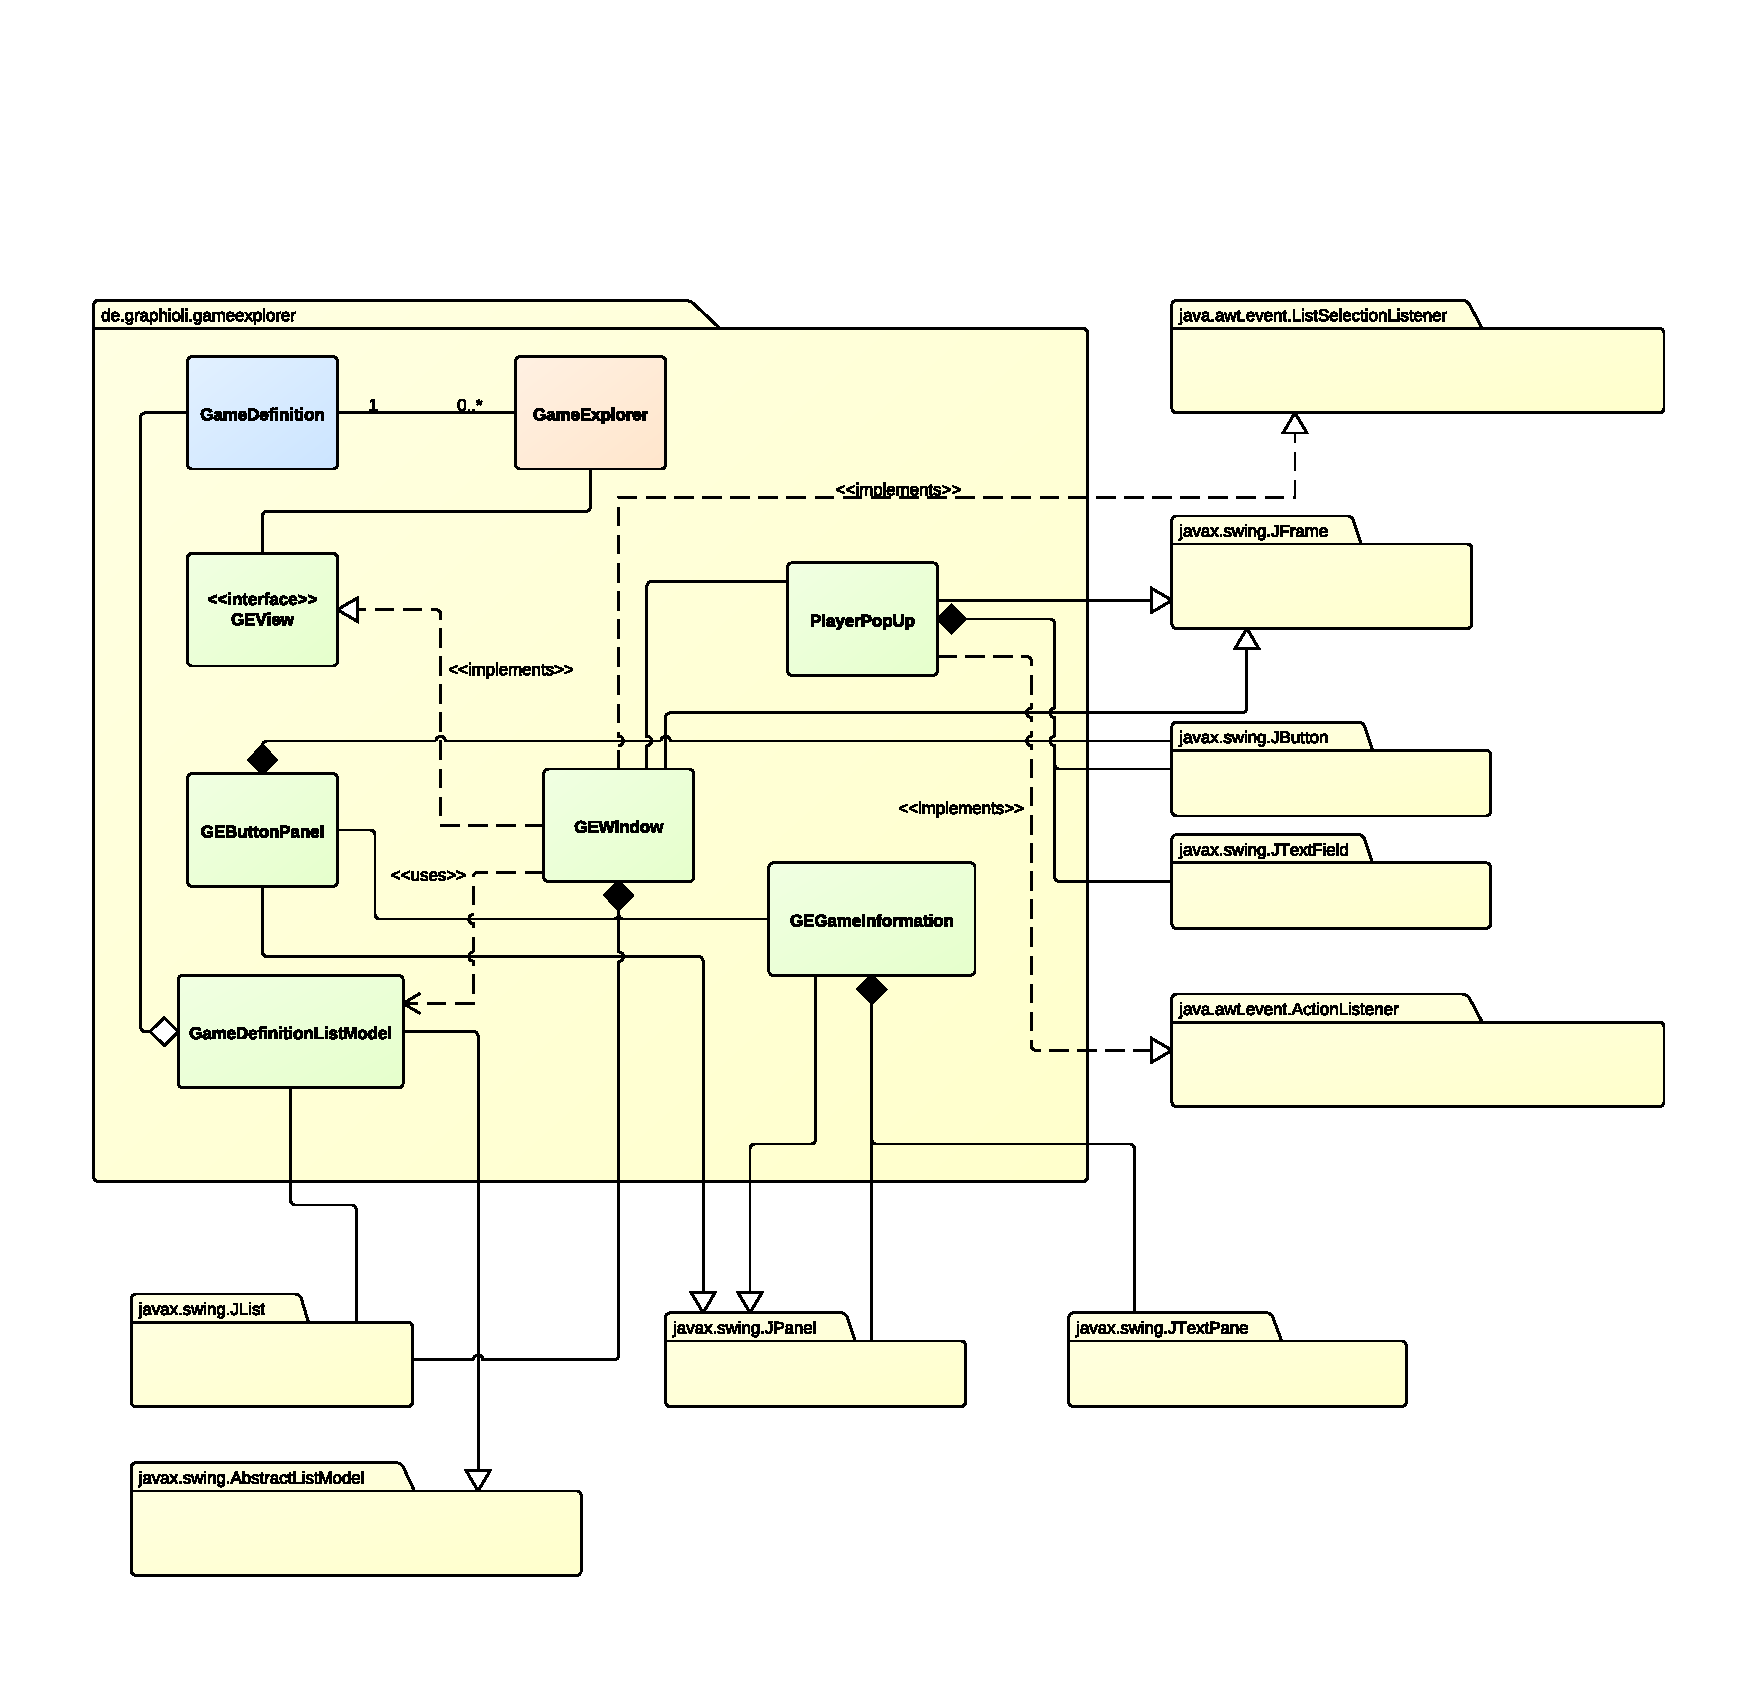
\includegraphics[page=1,width=\textwidth,keepaspectratio]{gameExplorerClassDiagram.pdf}
	\caption{GameExplorer class diagram.}
	\label{img:gameExplorerClassDiagram}
\end{figure}
\pagebreak

% GameExplorer
\class{GameExplorer}{gameexplorer}
The \texttt{GameExplorer} lists the available games and enables the user to select and start one of it.

\centerdash

\paragraph*{Method Summary}
\paragraph*{}
\begin{longtable}{Lp{10cm}}
	\startmethodtable
	\method{public}{GameExplorer(GameManager gameManager)}{ge:gameexplorer} \\
	& Creates a new \texttt{Game Explorer}. \\
	\method{private GameDefinition}{createGameDefinitionFromJSON(String jsonString)}{ge:creategamedefinitionfromjson} \\
	& Parses a \ref{cls:gamedefinition} from a given JSON string. \\
	\method{private Iterable<GameDefinition>}{scanGameFolder()}{ge:scangamefolder} \\
	& Scans the \texttt{Game Folder} for games and returns the \ref{cls:gamedefinition}s of the games in it. \\
	\method{public boolean}{selectGame(GameDefinition gameDef, Iterable<Player> players)}{ge:selectgame} \\
	& Calls the \ref{cls:gamemanager} to start the game of the given \ref{cls:gamedefinition} and with the given \ref{cls:player}s. \\
	\method{public boolean}{openHelpFile(GameDefinition gameDef)}{ge:openhelpfile} \\
	& Opens the help file of the given \ref{cls:gamedefinition}. \\
	\method{public Iterable<GameDefinition>}{getGameDefinitions()}{ge:getgamedefinitions} \\
	& Returns the \ref{cls:gamedefinition}s of this \texttt{GameExplorer}. \\
	\method{public GameDefinition}{getGameDefinitionAtIndex(int index)}{ge:getgamedefinitionatindex} \\
	& Returns the \ref{cls:gamedefinition} at the specific index. \\
	\hline
\end{longtable}

\pagebreak

% GameDefinition
\class{GameDefinition}{gamedefinition}
This class represents the game's definition, containing crucial information that is needed to start a game.

\centerdash
\paragraph*{Method Summary}
\paragraph*{}
\begin{longtable}{Lp{10cm}}
	\startmethodtable
	\method{public}{GameDefinition({params})}{gd:gamedefinition} \\
	& Creates a new \texttt{GameDefinition} with the specified parameters. \\
	\method{public String}{getName()}{gd:getname} \\
	& Returns the \texttt{name} of this \texttt{GameDefinition}, which is the name of the game. \\
	\method{public int}{getMaxPlayerCount()}{gd:getmaxplayercount} \\
	& Returns the maximum number of players for this specific game. \\
	\method{public int}{getMinPlayerCount()}{gd:getminplayercount} \\
	& Returns the minimum number of players for this specific game. \\
	\method{public String}{getGamePath()}{gd:getgamepath} \\
	& Returns the path of this specific game. \\
	\method{public String}{getDescription()}{gd:getdescription} \\
	& Returns the description of this specific game. \\
	\method{public String}{getFullyQualifiedClassName()}{gd:getfullyqualifiedclassname} \\
	& Returns the fully qualified class name (e.g. ``de.graphioli.game.GraphColoring'') of this specific game. \\
	\method{public BufferedImage}{getScreenshot()}{gd:getscreenshot} \\
	& Returns a \texttt{BufferedImage} that is this game's screenshot. \\
	\method{public File}{getLocalizedString()}{gd:getlocalizedstring} \\
	& Returns a \texttt{String} telling which language file should be used. \\
	\method{public URI}{getHelpFile()}{gd:gethelpfile} \\
	& Returns the \texttt{URI} that links to the help file of this game. \\
	\method{public Iterable<MenuItem>}{getMenu()}{gd:getmenu} \\
	& Returns an iterable list of \texttt{MenuItem}s that will be used to generate this game's custom \texttt{MenuBar}. \\
	\method{public int}{getHorizontalGridPointCount()}{gd:gethorizontalgridpointcount} \\
	& Returns the number of horizontal \ref{cls:gridpoint}s for this specific game. \\
	\method{public int}{getVerticalGridPointCount()}{gd:getverticalgridpointcount} \\
	& Returns the number of vertical \ref{cls:gridpoint}s for this specific game. \\
	\method{public boolean}{isDirectedGraph()}{gd:isdirectedgraph} \\
	& Returns whether the game's graph is directed. \\
	\hline
\end{longtable}

\pagebreak

% GameExplorerView (interface)
\interface{GEView}{geview}
This interface defines the methods the \ref{cls:gameexplorer} uses to communicate with its \gls{GUI}. \\

\centerdash

\paragraph*{Method Summary}
\paragraph*{}
\begin{longtable}{Lp{10cm}}
	\startmethodtable
	\method{public boolean}{registerController(GameExplorer gameExplorer)}{gev:registercontroller} \\
	& Registers the controller for the Game Explorer user interface. \\
	\method{public boolean}{generateView()}{gev:generateview} \\
	& Generates the user interface of the \ref{cls:gameexplorer}. \\
	\hline
\end{longtable}

\pagebreak

% GameExplorerWindow
\class{GEWindow}{gewindow}
\createindentedlist{java.lang.Object, java.awt.Component, java.awt.Container, java.awt.Window, java.awt.Frame, javax.swing.JFrame, de.graphioli.gameexplorer.GEWindow}
This class represents the main window of the \ref{cls:gameexplorer}. \\

\begin{description}
	\item[All Implemented Interfaces] \hfill \\
	\ref{cls:geview}, java.awt.event.ListSelectionListener
\end{description}

\centerdash

\paragraph*{Method Summary}
\paragraph*{}
\begin{longtable}{Lp{10cm}}
	\startmethodtable
	\method{public boolean}{generateView()}{gew:generateview} \\
	& Generates the graphical user interface of the \ref{cls:gameexplorer} (\ref{cls:gegameinformation}, \ref{cls:gebuttonpanel} and JList containing the \ref{cls:gamedefinitionlistmodel}). \\
	\method{public void}{valueChanged(ListSelectionEvent event)}{gew:valuechanged} \\
	& Called by the \texttt{JList} when its selection has changed to update the remaining graphical elements of this \texttt{GEWindow}. \\
	\method{public boolean}{openHelpFile()}{gew:openhelpfile} \\
	& Calls \ref{ge:openhelpfile} of \ref{cls:gameexplorer} with the \texttt{selectedGameDefinition}. \\
	\method{public boolean}{openPlayerPopUp()}{gew:openplayerpopup} \\
	& Creates and shows a \ref{cls:playerpopup} for player selection. \\
	\method{public boolean}{onPlayerPopUpReturn(Iterable<Player> players)}{gew:onplayerpopupreturn} \\
	& Called by the \ref{cls:playerpopup} when it has finished and triggers the start of the game. \\
	\hline
\end{longtable}

\pagebreak

% PlayerPopUp
\class{PlayerPopUp}{playerpopup}
\createindentedlist{java.lang.Object, java.awt.Component, java.awt.Container, java.awt.Window, java.awt.Frame, javax.swing.JFrame, de.graphioli.gameexplorer.PlayerPopUp}

Represents a pop-up window that is used to select the the number of players and their names for a game. \\
\begin{description}
	\item[All Implemented Interfaces] \hfill \\
	java.awt.event.ActionListener
\end{description}

\centerdash

\paragraph*{Method Summary}
\paragraph*{}
\begin{longtable}{Lp{10cm}}
	\startmethodtable
	\method{public}{PlayerPopUp(int minPlayer, int maxPlayer)}{ppu:playerpopup} \\
	& Creates a \texttt{PlayerPopUp}. \\
	\method{public void}{actionPerformed(ActionEvent event)}{ppu:gamedefinitionlistmodel} \\
	& Callback method for the Buttons, that creates the \ref{cls:player}s based on the input and calls \ref{gew:onplayerpopupreturn}. \\
	\hline
\end{longtable}

\pagebreak

% GameDefinitionListModel
\class{GameDefinitionListModel}{gamedefinitionlistmodel}
Represents a data model that provides the \texttt{JList} with its content. \\

\centerdash

\paragraph*{Method Summary}
\paragraph*{}
\begin{longtable}{Lp{10cm}}
	\startmethodtable
	\method{public}{GameDefinitionListModel(Iterable<GameDefinition> definitions)}{gdlm:gamedefinitionlistmodel} \\
	& Creates a new game definition list model with the given \ref{cls:gamedefinition}s. \\
	\method{public Object}{getElementAt(int index)}{gdlm:getgamedefinitionatindex} \\
	& Returns the name of the \ref{cls:gamedefinition} at the given index so the \texttt{JList} can display it. \\
	\hline
\end{longtable}

\pagebreak

% GameExplorerGameInformation
\class{GEGameInformation}{gegameinformation}
\createindentedlist{java.lang.Object, java.awt.Component, java.awt.Container, javax.swing.JComponent, javax.swing.JPanel, de.graphioli.gameexplorer.GEGameInformation}

Organizes the output of the screenshot and the description of the game. \\

\centerdash

\paragraph*{Method Summary}
\paragraph*{}
\begin{longtable}{Lp{10cm}}
	\startmethodtable
	\method{public boolean}{setDescription(String description)}{gegi:setdescription} \\
	& Sets the description of the game and updates the display \\
	\method{public boolean}{setScreenshot(BufferedImage screenshot)}{gegi:setscreenshot} \\
	& Sets the screenshot of the game and updates the display \\
	\hline
\end{longtable}

\pagebreak

% GameExplorerButtonPanel
\class{GEButtonPanel}{gebuttonpanel}
\createindentedlist{java.lang.Object, java.awt.Component, java.awt.Container, javax.swing.JComponent, javax.swing.JPanel, de.graphioli.gameexplorer.GEButtonPanel}

Organizes buttons and listens to them calling the specific methods in the \ref{cls:gewindow}. \\
\begin{description}
	\item[All Implemented Interfaces] \hfill \\
	java.awt.event.ActionListener
\end{description}

\centerdash

\paragraph*{Method Summary}
\paragraph*{}
\begin{longtable}{Lp{10cm}}
	\startmethodtable
	\method{public boolean}{setButtonsActive(boolean isActive)}{gebp:setbuttonsactive} \\
	& Sets the buttons (in)active. \\
	\method{public boolean}{actionPerformed(ActionEvent event)}{gebp:actionperformed} \\
	& Invokes if a button is clicked and calls the specific methods in the \ref{cls:gewindow} for the selected button. \\
	\hline
\end{longtable}

\section{Sequence Diagrams}

\begin{figure}[h]
	\centering
	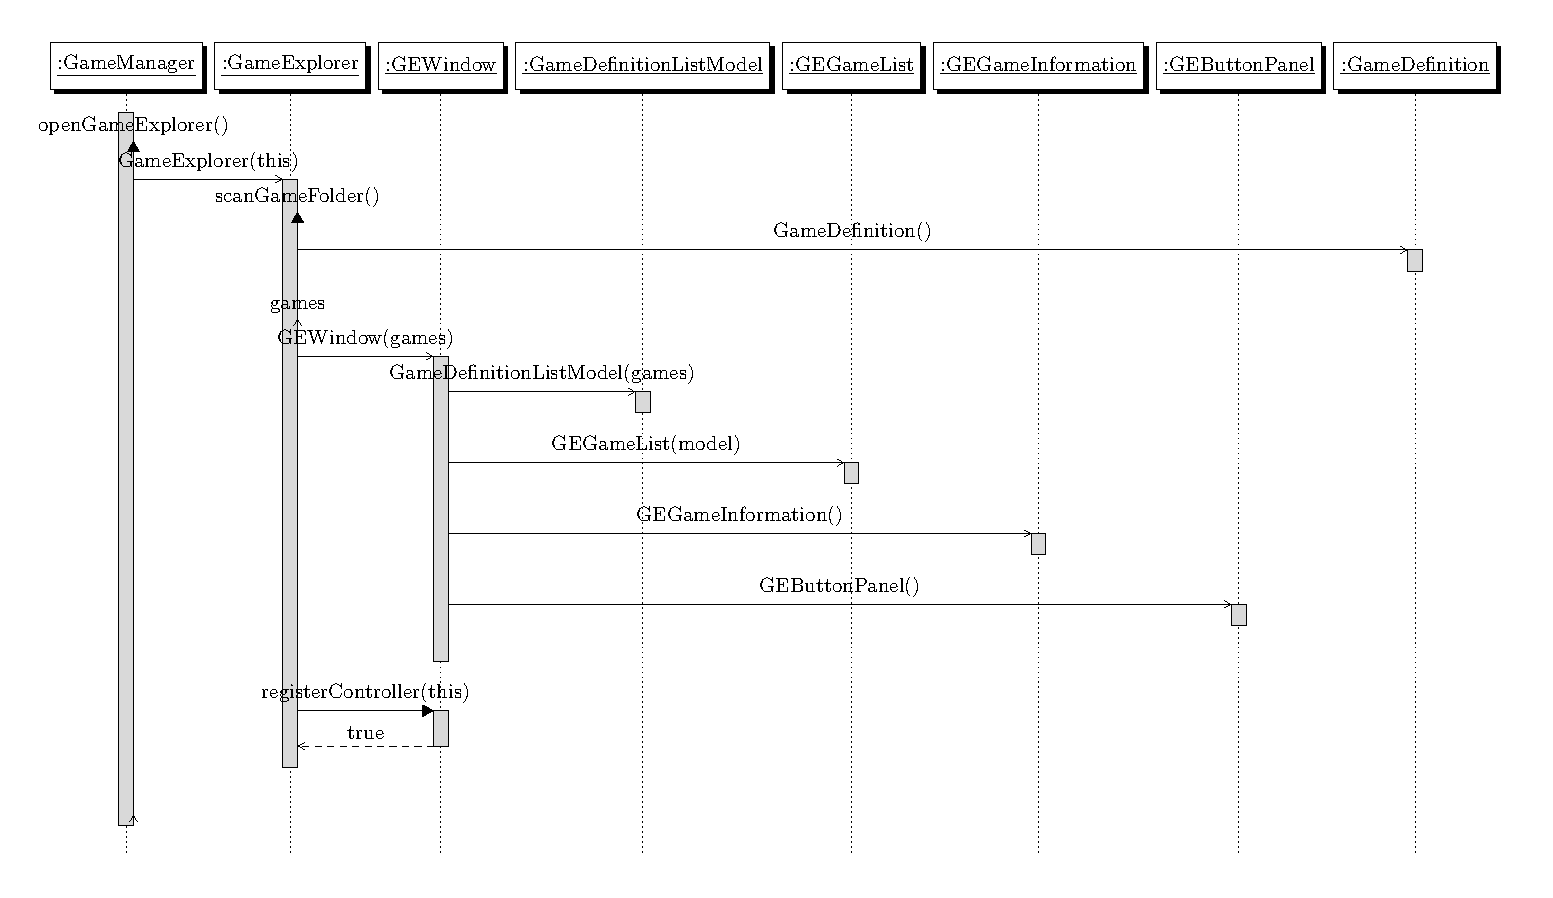
\includegraphics[angle=90,height=0.72\textheight,keepaspectratio]{1-seqGameExplorerInitialization.pdf}
	\caption{Sequence diagram showing the process of initializing the \gameexplorer.}
	\label{img:seqGameExplorerInitialization}
\end{figure}

\begin{figure}[h]
	\centering
	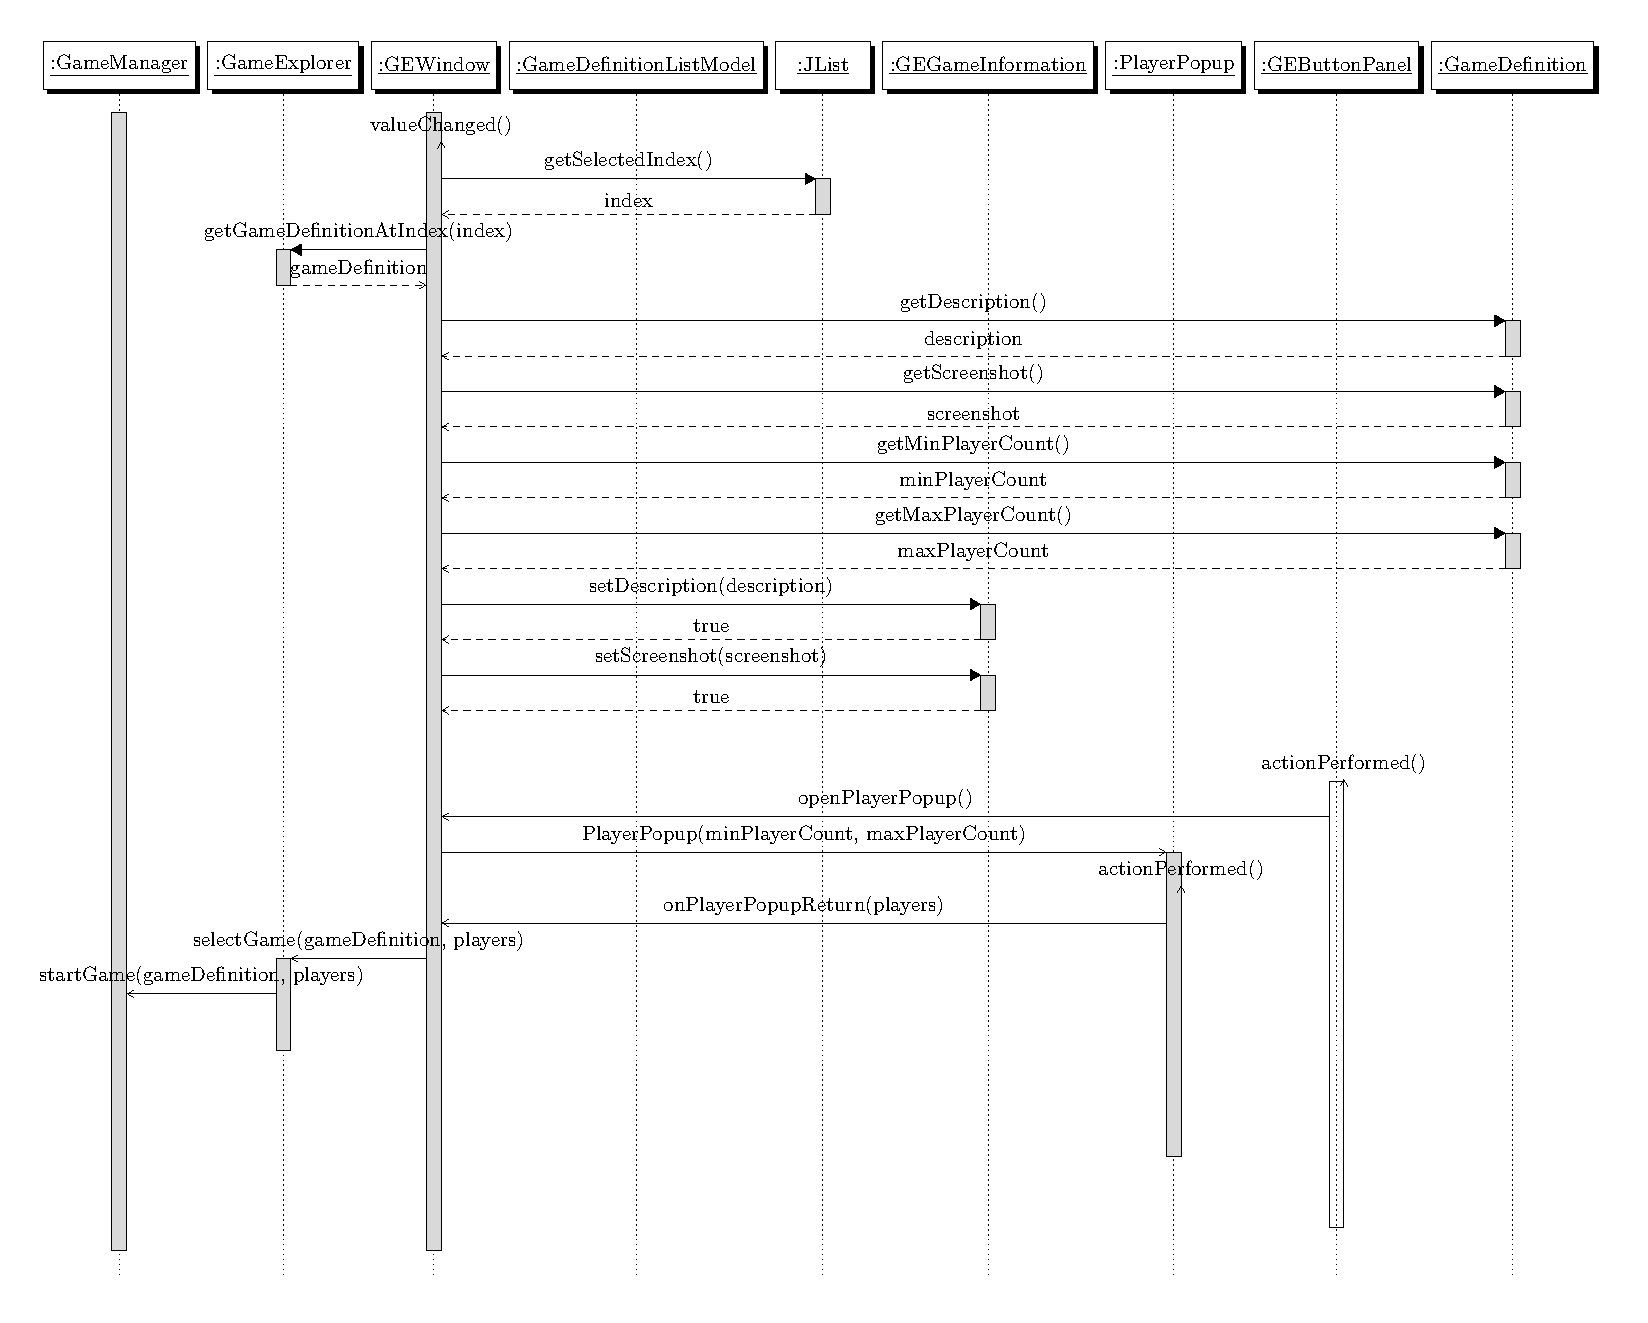
\includegraphics[angle=90,height=0.8\textheight]{2-seqSelectGame.pdf}
	\caption{Sequence diagram showing the process of selecting a game with an initialized \gameexplorer.}
	\label{img:seqSelectGame}
\end{figure}

\begin{figure}[h]
	\centering
	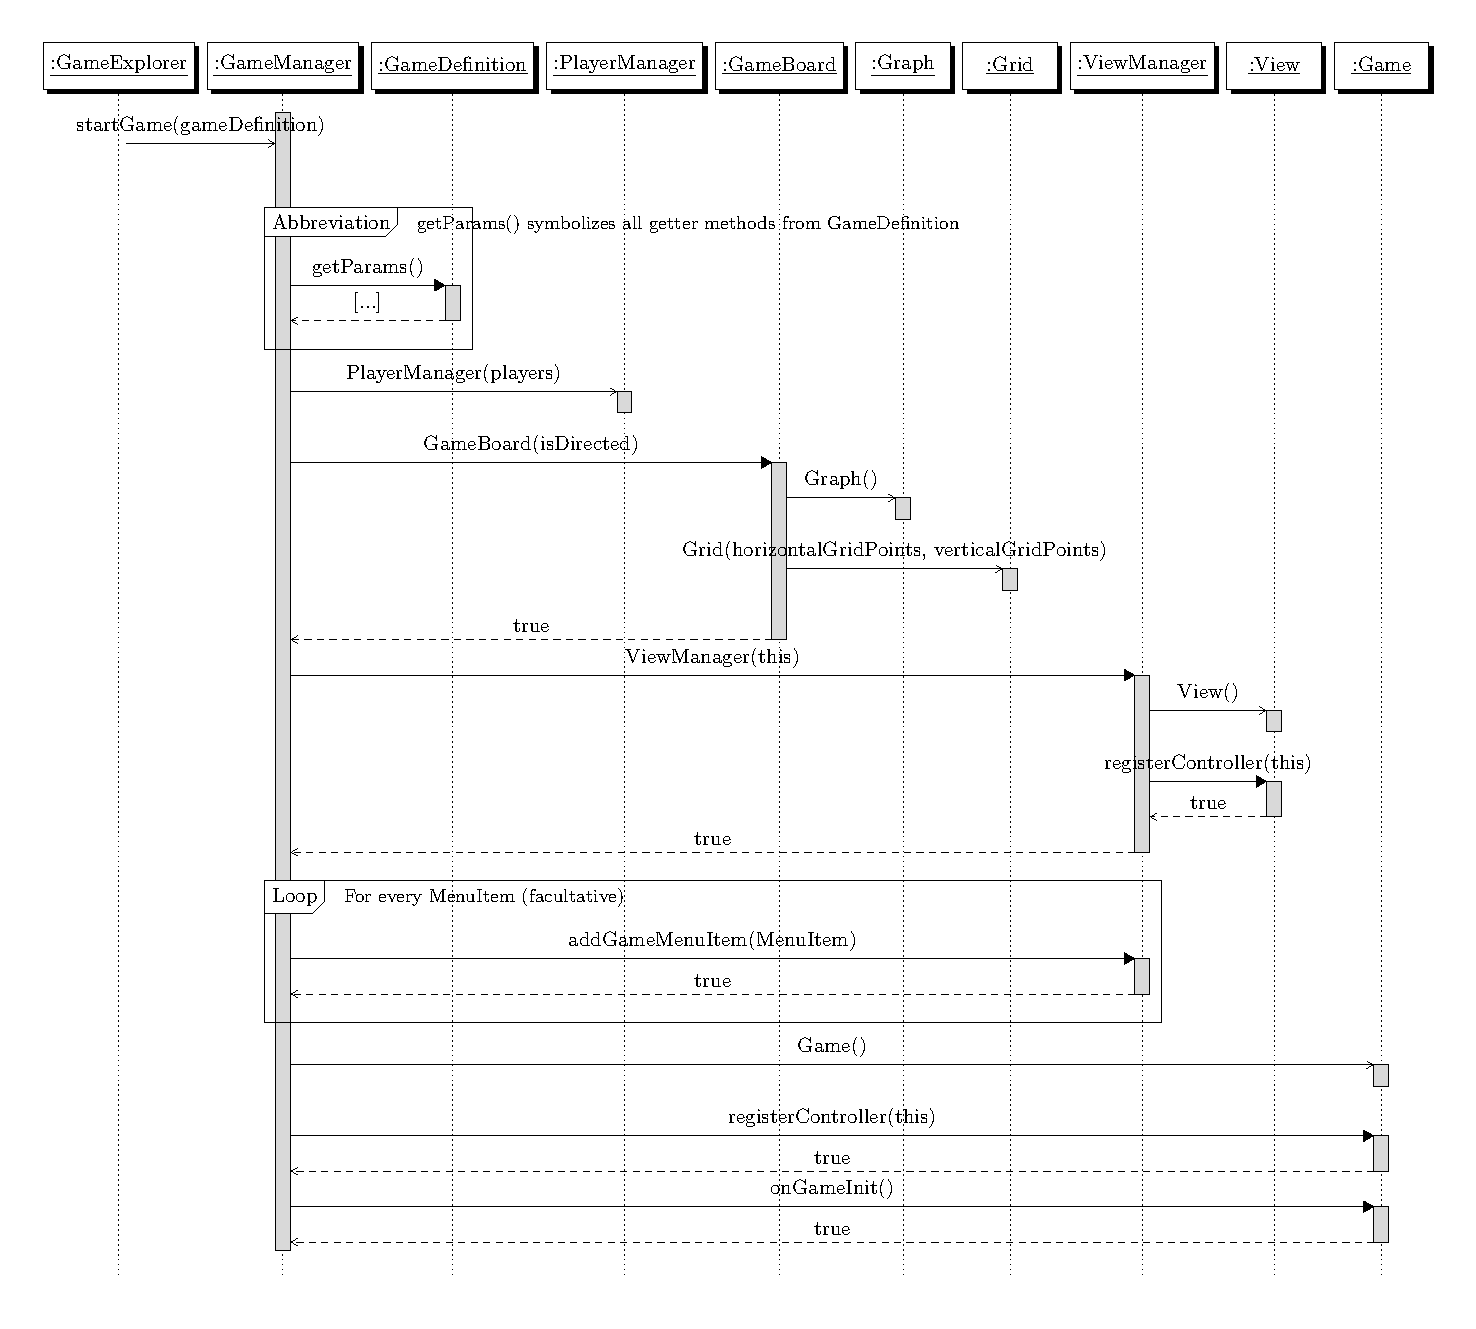
\includegraphics[angle=90,width=1\textwidth]{3-seqGameInitialization.pdf}
	\caption{Sequence diagram showing the process of a game's initialization.}
	\label{img:seqGameInitialization}
\end{figure}

\begin{figure}[h]
	\centering
	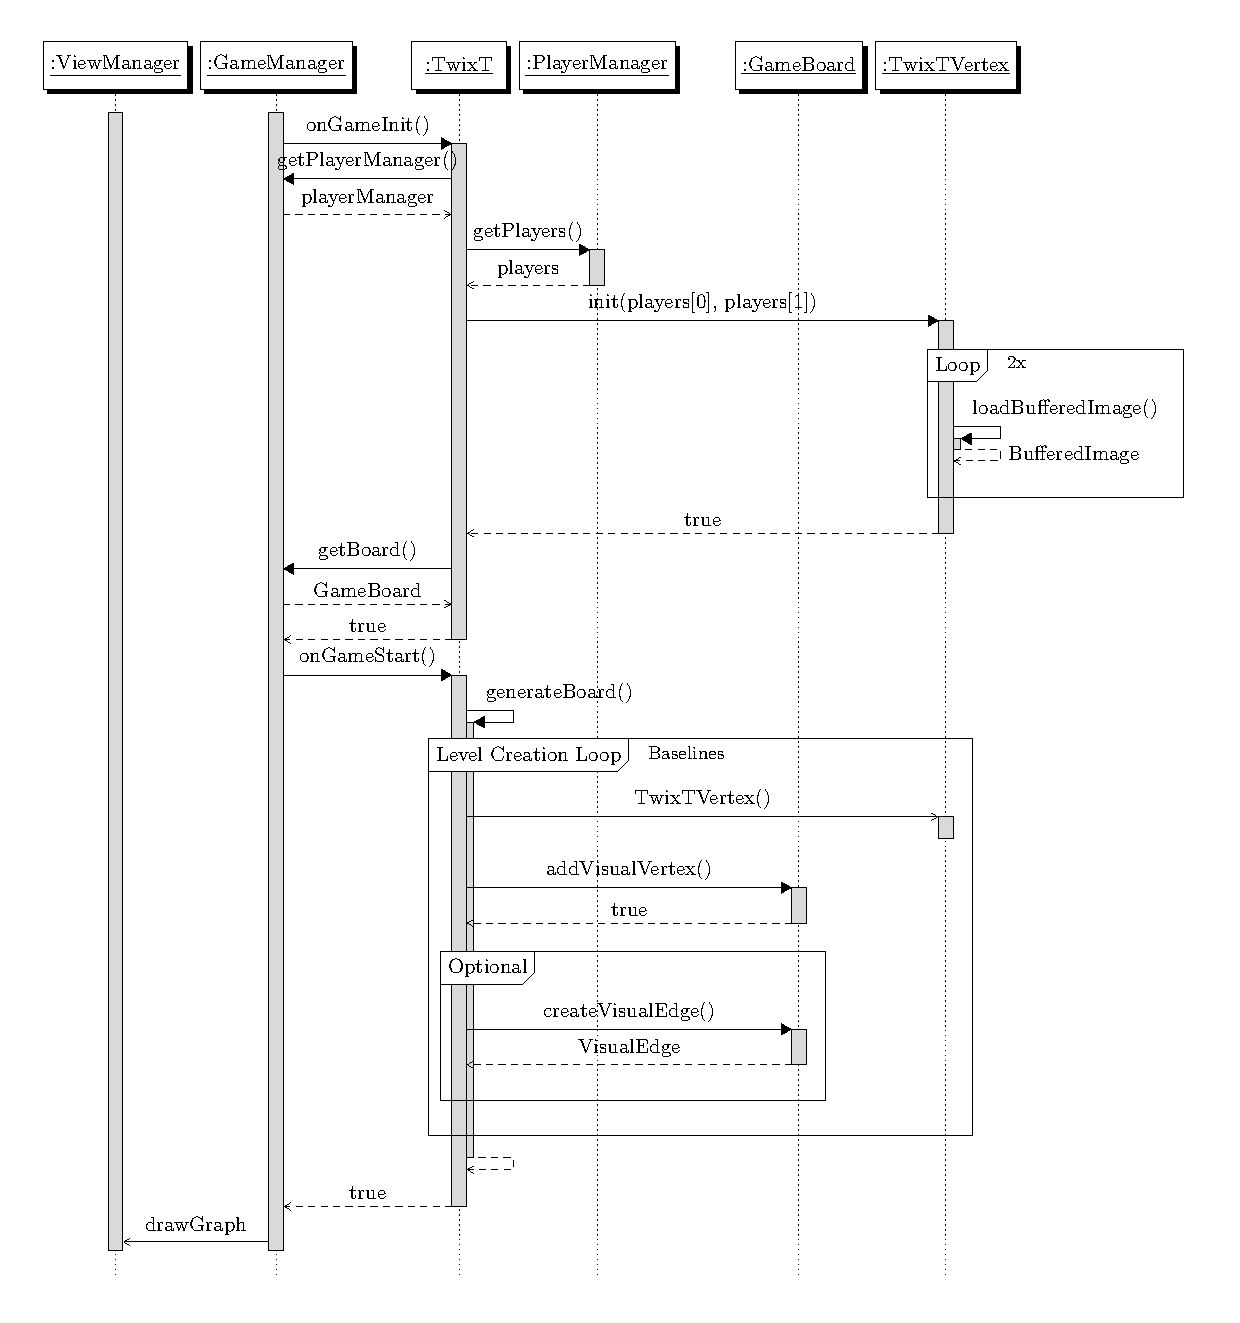
\includegraphics[width=1\textwidth]{4-seqTwixtInitialization.pdf}
	\caption{Sequence diagram showing the process of initializing a new \twixt game.}
	\label{img:seqTwixtInitialization}
\end{figure}

\begin{figure}[h]
	\centering
	\includegraphics[page=2,angle=90,width=1\textwidth]{5-seqTwixt.pdf}
	\caption{Sequence diagram showing the process of creating vertices and edges in the game implementation \twixt.}
	\label{img:seqTwixt}
\end{figure}

\begin{figure}[h]
	\centering
	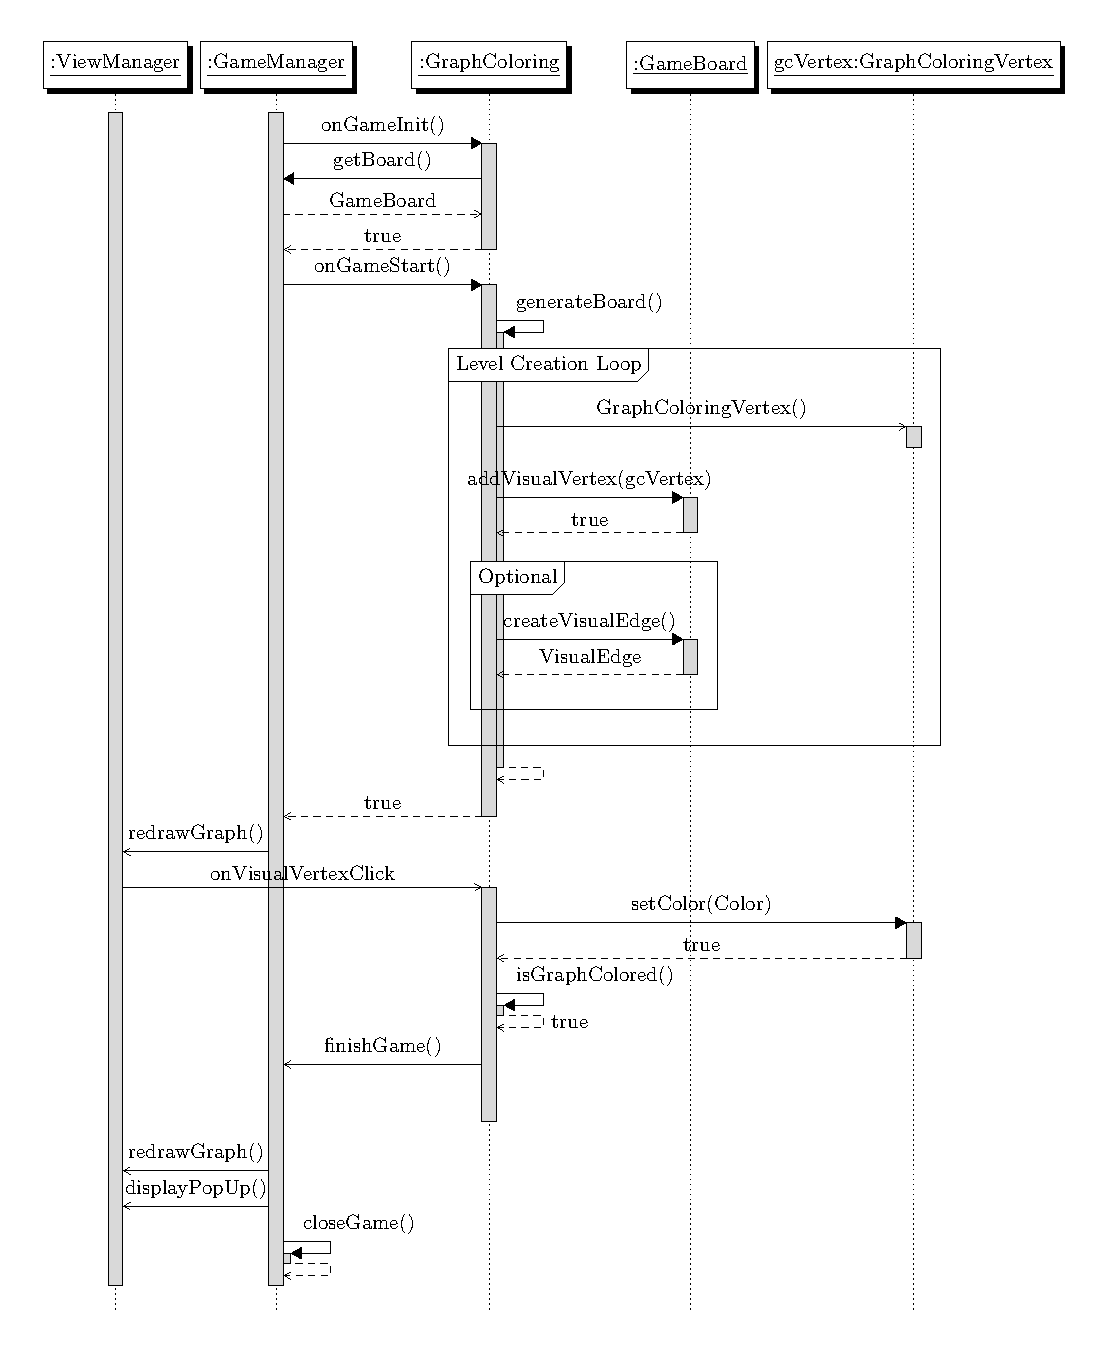
\includegraphics[width=1\textwidth]{6-seqGraphcoloringInitialization.pdf}
	\caption{Sequence diagram showing the process of initializing, playing and winning a \graphcoloring game.}
	\label{img:seqGraphcoloringInitialization}
\end{figure}

\begin{figure}[h]
	\centering
	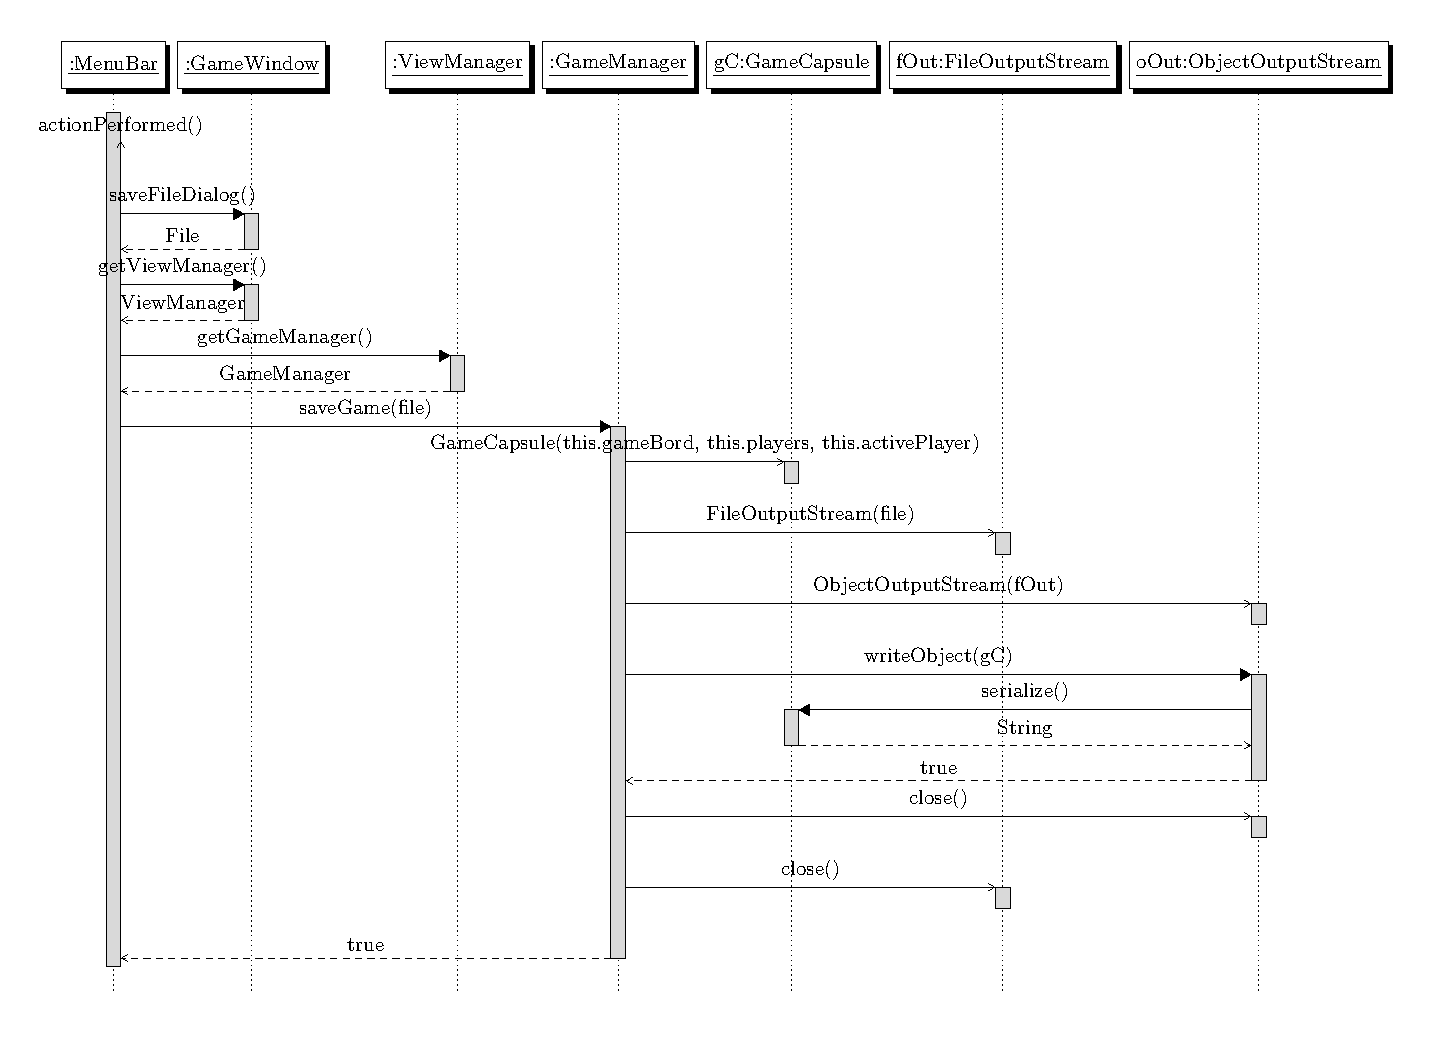
\includegraphics[angle=90,width=1\textwidth]{7-seqSaveGame.pdf}
	\caption{Sequence diagram showing the process of saving a game.}
	\label{img:seqSaveGame}
\end{figure}

\begin{figure}[h]
	\centering
	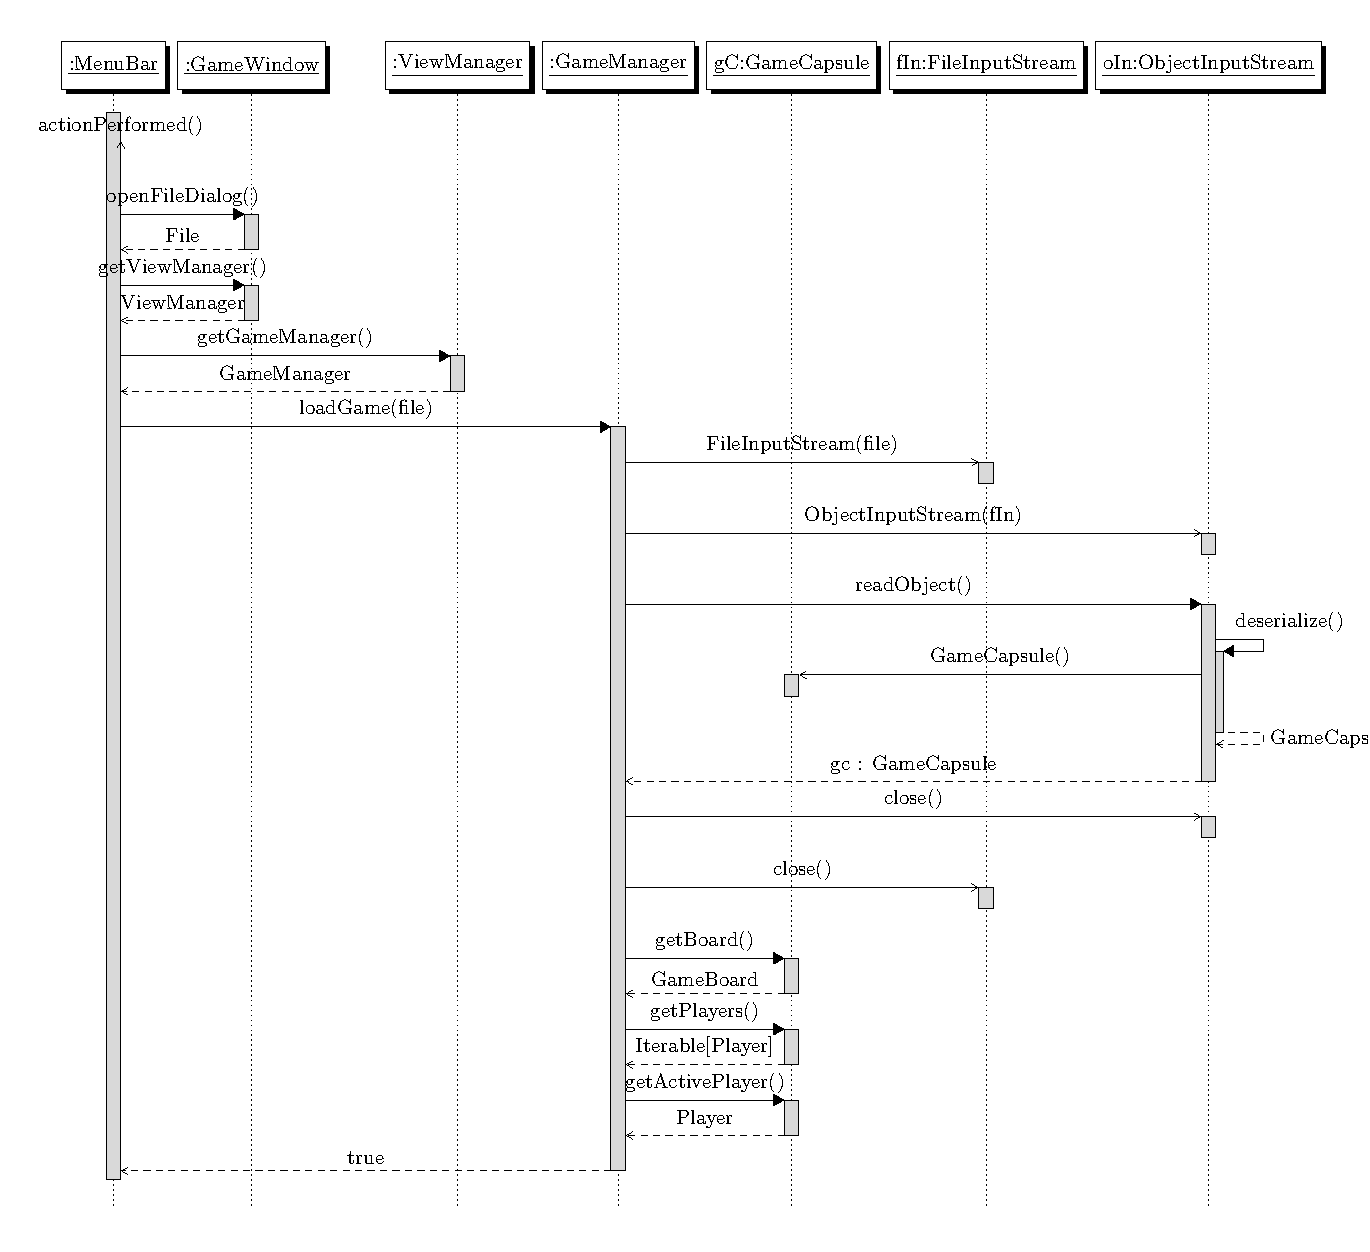
\includegraphics[angle=90,width=1\textwidth]{8-seqLoadGame.pdf}
	\caption{Sequence diagram showing the process of loading a game.}
	\label{img:seqLoadGame}
\end{figure}

\begin{figure}[h]
	\centering
	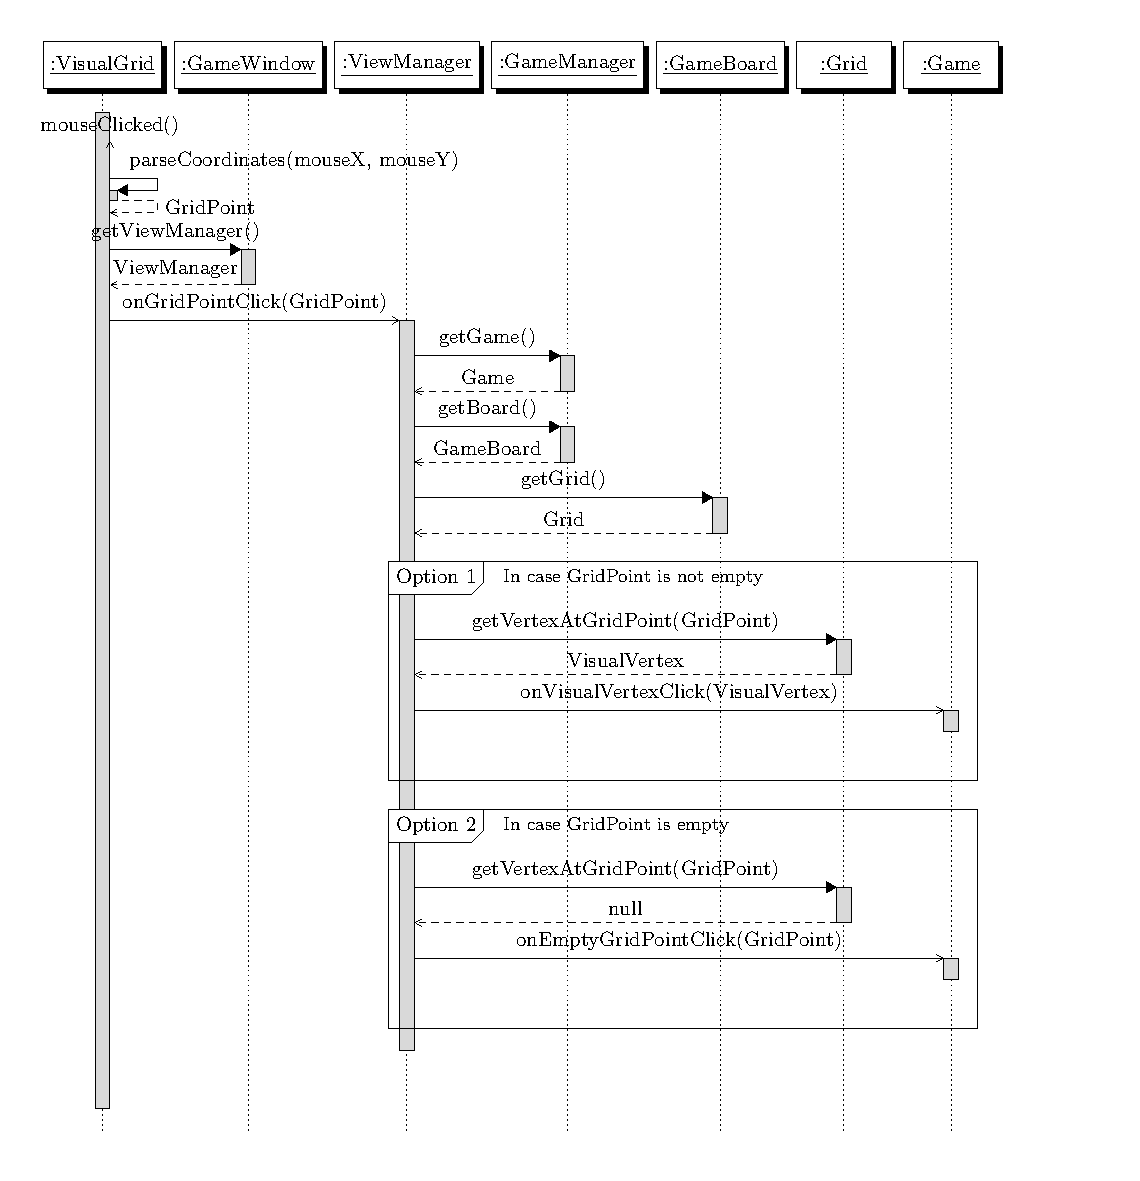
\includegraphics[angle=90,width=1\textwidth]{9-seqClickAction.pdf}
	\caption{Sequence diagram showing the actions performed after a mouse click event.}
	\label{img:seqClickAction}
\end{figure}
\section{Miscellaneous}
\subsection{Game property file}

\begin{lstlisting}[caption=An example of a property file]
/* This is an example property file for the 'Dummy' game. */

{
    "game": [{
        "name": "Dummy",
        "gamePath": "..path/to/dummy/",
        "fullyQualifiedClassName": "de.graphioli.game.Dummy",
        "description": "This is a description for the Dummy game",
        "screenshot": "./screenshot.png",
        "languageFile": "./language_en.txt",
        "helpFile": "../helpFile.pdf",
        "maxPlayerCount": 1,
        "minPlayerCount": 4,
        "menuItem": [{
            "save": 1,
            "load": 2,
            "exit": 3
        }],
        "horizontalGridPointCount": 100,
        "verticalGridPointCount": 100
    }]
}
\end{lstlisting}

\section{Glossary}

\end{document}
